\ProvidesFile{rutitlepage.dtx}[2022/02/21 v3.0 Radboud University Titlepage]
\documentclass{ltxdoc}
\newcommand{\messagespace}{\text{$\mathcal{M}$}}
\newcommand{\messageinstance}{\text{$m$}}
\newcommand{\ciphertextspace}{\text{$\mathcal{C}$}}
\newcommand{\ciphertextinstance}{\text{$c$}}
\newcommand{\associateddataspace}{\text{$\mathcal{A}$}}
\newcommand{\associateddatainstance}{\text{$a$}}
\newcommand{\tagspace}{\text{$\mathcal{T}$}}
\newcommand{\taginstance}{\text{$t$}}
\newcommand{\keyspace}{\text{$\mathcal{K}$}}
\newcommand{\keyinstance}{\text{$k$}}
\newcommand{\noncespace}{\text{$\mathcal{N}$}}
\newcommand{\nonceinstance}{\text{$n$}}
\newcommand{\lockspace}{\text{$\mathcal{L}$}}
\newcommand{\lockinstance}{\text{$l$}}
\newcommand{\users}{\text{$N$}}
\newcommand{\user}{\text{$j$}}
\newcommand{\adversary}{\text{$A$}}
\newcommand{\sample}{\text{$\leftarrow$}}
\newcommand{\result}{\text{$\leftarrow$}}
\newcommand{\concatinate}{\text{$\|$}}

\newcommand{\advantage}[2]{\textbf{Adv}$_{\text{#1}}^{\text{#2}}$ }
\newcommand{\probabilityblock}[4]{\text{$|\text{Pr}[\text{#1}_{\text{#2}}^{\text{#3}}] - \text{Pr}[\text{#1}_{\text{#2}}^{\text{#4}}]|$}}

\newcommand{\pkc}{\text{Hybrid Encryption in a Multi-user Setting, revised}}
\newcommand{\gcrec}{\text{Generic Composition Reconsidered}}

\newcommand{\x}{\text{x}}
\usepackage{a4wide}
\usepackage{float}
\usepackage{graphicx}
\usepackage{array}
\usepackage[utf8]{inputenc}
\usepackage{rutitlepage}
\usepackage{fancyhdr}
\usepackage[style=ieee]{biblatex}
\usepackage[operators]{cryptocode}
\usepackage{amssymb}
\usepackage{amsthm}
\usepackage{amsmath}
\addbibresource{cryptobib/crypto.bib}
\addbibresource{references.bib}
\GetFileInfo{rutitlepage.dtx}
\newtheorem{theorem}{Theorem}

\pagestyle{fancy}
\fancyhf{}
\lhead{Bachelor Thesis}
\rhead{Page \thepage}

\title{Bachelor Thesis Stijn Vandenput}
\author{stijnvandenput }

\begin{document}
\maketitleru[
    layout=traditional,
    authors={Stijn Vandenput},
    authorstext={Author:},
    nextpagenr={-1},
    institution={Radboud University},
    others={Supervisors:}{Martijn Stam\\Bart Mennink},
    course={Bachelor Thesis},
    title={TBD}]

\section*{Abstract}

\pagenumbering{roman}
\newpage
\tableofcontents

\newpage
\pagenumbering{arabic}

\section{Introduction}
To implement public-key encryption, a hybrid paradigm is typically followed: To encrypt a message, an ephemeral key is generated using a randomized key encapsulation mechanism (KEM). This key is then used to encrypt the message using a deterministic data encapsulation mechanism (DEM). Both the KEM and DEM output their own ciphertexts, which are concatenated to form the public-key encryption ciphertext. Classical analysis of DEMs considers a single user. Because of this, the security bounds of these analysis do not always transfer to the real worlds where you can have millions of users. To make sure the security bounds are also good if you have many users, you can use larger ephemeral keys. Although using larger keys for DEMs is generally safer, expanding the size of the key is not always a viable option. This might be due to limitations in computing power or memory, or due to security primitives having fixed key sizes. Giacon, Kiltz and Poettering, henceforth \gkp{}, propose augmentation using locks (originally called tags, but renamed to locks here to avoid overloaded terms) as an alternative solution to key expansion in a multi-user setting \cite{PKC:GiaKilPoe18}. Augmentation with locks works by giving the security primitive an additional input field, called the lock, to distinguish multiple users using the same key. The augmentation can improve security in a multi-user setting, without the need to expand the key.
\\\\
After defining this augmentation, GKP apply the augmentation to a DEM and a MAC function, to create an augmented DEM (ADEM) and an augmented MAC (AMAC). These two are combined to construct an authenticated encryption primitive following the generic encrypt-then-MAC composition from Bellare and Namprempre \cite{AC:BelNam00}. This composition is proven secure whenever the underlying ADEM and AMAC are secure. The generic composition of authenticated encryption has been revised by Namprempre, Rogaway and Shrimpton \cite{EC:NamRogShr14}, which we henceforth call \nrs{}. In this revision, the generic composition using a MAC function and a deterministic encryption primitive is more thoroughly investigated. They shine light on the fact that the kind of encryption primitive used has a impact on which kinds of generic compositions are secure. When using a nonce-based authenticated encryption primitive and a MAC function, the encrypt-and-MAC, the encrypt-then-MAC and the MAC-then-encrypt are proven to be secure whenever the underlying primitives are secure.
\\\\
Although the ADEM+AMAC composition given by GKP is secure, it is not clearly defined as authenticated encryption primitive. As a result, its security is evaluated as a DEM, not as an authenticated encryption primitive. Additionally, only the encrypt-then-MAC composition is considered by GKP and it is not shown if other composition methods could be secure. In this thesis, generic composition of authenticated encryption using locks is more thoroughly investigated. We formally compare the constructions and the notation from NRS and GKP (Chapter 3). To evaluate generic composition using locks, we define a new cryptographic primitive which we analyze in a multi-user setting (Chapter 4). Using the knowledge from NRS, three generic compositions (encrypt-and-MAC, encrypt-then-MAC and MAC-then-encrypt) of this primitive are considered, all using a lock-based encryption primitive and a lock-based MAC function (Chapter 5). These compositions are then proven to be secure, whenever the underlying primitives are secure (Appendix A).

\section{Preliminaries}
In this section we will explain several concepts important to the rest of our work, as well as some general notation.

\subsection{General Notation}
Strings are binary and bit-wise, the set of all strings is $\{0,1\}^\ast$. The length of $x$ is written as $\abs{x}$, the concatenation of $x$ and $y$ as $x$ \concatinate{} $y$, $a$ being the result of $b$ as $a$ \result{} $b$, and taking a uniform random sampling from set $z$ and assigning it to $x$ as $x$ \sample{} $z$. We write \users{} for the number of users and allow a single type of error message written as \invalid. Any tuple containing \invalid{} will be \invalid{} as well. We define the following spaces, all of them being subsets of the set of all strings: nonempty key space \keyspace{}, lock space \lockspace{}, nonce space \noncespace{}, message space \messagespace{}, ciphertext space \ciphertextspace, tag space \tagspace{}, and associated data space \associateddataspace{}. Unless stated otherwise, \messagespace{} contains at least two strings, and if \messagespace{} or \associateddataspace{} contains a string of length $x$, it must contain all strings of length $x$. There are no further constraints on these spaces.

\subsection{Authenticated Encryption}
Two different security requirements are data privacy, the insurance that data cannot be viewed by an unauthorized party, and data integrity, the insurance that data has not been modified by an unauthorized party. Authenticated encryption combines both of these security requirements into one and ensures both data privacy and integrity. A basic authenticated encryption scheme consists of a encryption call and a decryption call. The encryption call takes a message and a key to a self-authenticating ciphertext. The decryption call takes a self-authenticating ciphertext and a key to a message. Some authenticated encryption schemes allow an additional input AD, short for associated data. The associated data is specifically required to not have data privacy but does require data integrity. Authenticated encryption schemes that support AD are called AEAD schemes.

\subsection{Message Authentication}
Message authentication can be done using a message authentication code, MAC for short. A basic MAC function takes a message and key and outputs a tag which authenticates the message. Some MAC functions also have a verification call that takes a message, key and tag and outputs either \codetrue{} or \codefalse. A MAC function can have different security requirements. It is said to be PRF secure when it is infeasible to distinguish the output tag from the result of a pseudo-random function that takes all message-key pairs to the tag space. A MAC is said to be unforgeable when it is infeasible to create a valid message-tag pair without knowledge of the secret key. A PRF secure MAC is also unforgeable, given the tag space is big enough, while a unforgeable MAC is not necessarily PRF secure.

\subsection{Nonces and Locks}
A basic deterministic encryption scheme takes a message and key as input, and outputs a ciphertext. Using this encryption scheme, a message encrypted under the same key leads to the same ciphertext. Both GPK (Giacon, Kiltz and Poettering) and NRS (Namprempre, Rogaway and Shrimpton) resolve this by giving the encryption scheme an additional argument. GKP uses locks while NRS uses nonces. Although nonces and locks look similar, their purpose and exact working differ leading to different use cases. Most notably, nonces are useful when one user is allowed  to encrypt multiple messages and locks are only useful when there are multiple users.

\paragraph{Nonces}
Using a basic deterministic encryption scheme, a message encrypted twice by the same user results in the same ciphertext. This can leak information about the message, which can be prevented by using a nonce. A nonce is a number that is assumed to only be used once per user to encrypt a message. Whenever a message is encrypted twice with the same key, but with two different nonces, the resulting ciphertexts should be indistinguishable from two ciphertexts corresponding to two different messages. As a result, it is infeasible for an adversary to guess if a message has been sent multiple times. The adversary is usually allowed to let a user decrypt multiple messages with one nonce. Nonces are only used when a user uses its key multiple times, as otherwise a message will never be encrypted by the same user twice.

\paragraph{Locks}
Using a basic deterministic encryption scheme, a message encrypted by two users that have the same key results in the same ciphertext. This can leak information about the secret keys used, which can be prevented by using locks. Whereas nonces are bound to the message, locks are bound to the user. Each user has one lock, provided the users have one key each, and will encrypt all their messages using that lock. Whenever a message is encrypted twice with the same key, but with two different locks, the resulting ciphertexts should be indistinguishable from two ciphertexts corresponding to two different messages. As a result, it is infeasible for an adversary to see when two users have a key collision unless locks collide as well. To prevent collisions in locks, we assume locks to be globally unique. The adversary is usually only allowed to let a user decrypt messages with the correct lock. Locks are only used in a multi-user setting, as key collision is impossible when there is only one user.  

\subsection{Security Notions}
The security of a cryptographic construction can be modeled as a distinguishing advantage. When doing this, different security notions are formed based on what you distinguish on. To understand NRS and GKP and how they differ, it is important to understand which security notions they use, all the relevant notions are written below.

\paragraph{Active of Passive}
Security can be modeled against an passive or an active attacker. An passive attacker can only read the messages while an active attacker can also alter the messages. An passive attacker can be modelled using a chosen plaintext attack, CPA for short. In this model, the adversary can choose the plaintext that is encrypted, but not the ciphertext that is decrypted. An active attacker can be modelled using a chosen ciphertext attack, CCA for short. In this model, the adversary can choose the plaintext that is encrypted, as well as the ciphertext that is decrypted. Shorthand notations for the two is IND-CPA and IND-CCA, respectively. IND-CCA implies IND-CPA, but not the other way around. Both GKP and NRS model the authenticated encryption primitive using IND-CPA and the underlying encryption primitive using IND-CCA.

\paragraph{\$ or Left-or-right}
Left-or-right-indistinguishablility refers to a situation where the adversary gives two messages, and is given a ciphertext. The adversary has to guess which of the two messages corresponds to the ciphertext. \$-indistinguishablility refers to a situation where the adversary is given access to either the real construction, or to a lazily sampled random function \$. This random function returns a random string with the same length as the ciphertext would have. The adversary has to guess which of these two it has access to. As long as the length of the ciphertext only depends on the length of the message, not its content, IND-\$ implies IND-LOR, but not the other way around. IND-\$ is used by GPK and IND-LOR is used by NRS.

\noindent\\
Both of these are separate dimensions and they can be combined into 4 different notions. For example IND-\$-CCA refers to a situation where the adversary has to distinguish between the real construction, or a random function while being able to choose both the plaintext that is encrypted and the ciphertext that is decrypted.

\paragraph{Game Based Security Notions}
These security notions can be written in a game-based format, using pseudocode instead of text. As a example, the IND-\$-CPA game of a nonce-based encryption scheme can be found in Figure \ref{fig: nE-IND game}. A challenge bit $b$ is given to the game, in this case $b$ signals whether we are in the real or the ideal world. The adversary guesses this bit and returns $b'$, signaling its guess for $b$. In addition, the adversary can have access to oracles. In our example there is only one oracle that takes a nonce and a message. Using game based notation, you can clearly write out all the limitations. For example, the limitation that nonces cannot be reused is modeled by lines 0, 5 and 6. Lines 8 and 9 model how the random function \$ behaves. These limitations could be written out in text based format as well but when there are multiple limitations, writing it out in a game based format can make both the security notion, as well as the security proofs, more comprehensible and precise.

\subsection{Security Proofs of Generic Composition}
To prove the security of a generic composition we use a security reduction. To define the reduction we bind the advantage of the generic composition by terms of the advantages of the underlying primitives. To do this we show that an advantage on the generic composition can be leveraged to gain an advantage on the underlying primitives. In other words, we prove that if we can break the security of the generic composition, then we can break the security of one of the underlying primitives. After proving this, we can conclude the composition is secure as long as the underlying primitives are secure. The security reduction is said to be tight when its security does not depend on the attack and lose when its security does depend on the adversary’s attack. 

\section{\nrs{} and \gkp{} in Detail}
In this section we explain the parts from \gkp{} and \nrs{} important to our work. Afterwards, a comparison is made between the two. Some notations will be different from the original papers for improved consistency. What are called tags by \gkp, we will call locks instead to avoid confusion with the output of MAC functions and we call the output of the AMAC the tag instead of the ciphertext. The security notions from \nrs{} are converted to a game-based format using insights from \cite{USENIX:CrAlJaZh23} in order to better match the notation from \gkp{} and be more adaptable to a multi-user setting. The security games are only explained briefly in this section, a more in-depth explanation of the relevant constructs can be found in section \ref{sec: lAE security model}.

\subsection{\nrs}
Three generic ways to compose an authenticated encryption scheme are discussed in a paper written by Bellare and Namprempre \cite{AC:BelNam00}: encrypt-then-MAC, encrypt-and-MAC and MAC-then-encrypt. In this paper, encrypt-then-MAC is considered the only secure composition when using probabilistic encryption as a building block. \nrs{} notes that the type of encryption scheme used influences which one of these compositions are secure. The constructions are generalized to using nonce-based encryption,  nA for short, and a PRF secure MAC function as a building blocks to create nonce-based authenticated encryption schemes, nAEs for short. Using these blocks, all three constructions are proven secure. Additionally, NRS add Associated data (AD) to the authenticated encryption primitive.

\subsubsection{Primitives}
\paragraph{nE}
A nonce-based encryption scheme is defined by a triple $\mathit{\Pi}$ = $(\keyspace{},\text{E},\text{D})$. Deterministic encryption algorithm E takes three inputs $(\keyinstance,\nonceinstance,\messageinstance)$ and outputs a value \ciphertextinstance, the length of \ciphertextinstance{} only depends the length of \keyinstance, \nonceinstance{} and \messageinstance. If, and only if, $(\keyinstance,\nonceinstance,\messageinstance)$ is not in $\keyspace \times \noncespace \times \messagespace$, \ciphertextinstance{} will be \invalid. Decryption algorithm D takes three inputs $(\keyinstance,\nonceinstance,\ciphertextinstance)$ and outputs a value \messageinstance. Both E and D are required to satisfy correctness (if E$(\keyinstance,\nonceinstance,\messageinstance)$ $= \ciphertextinstance \neq \invalid$, then D$(\keyinstance,\nonceinstance,\ciphertextinstance)$ = \messageinstance) and tidiness (if D$(\keyinstance,\nonceinstance,\ciphertextinstance)$ $= \messageinstance \neq \invalid$, then E$(\keyinstance,\nonceinstance, \messageinstance)$ = \ciphertextinstance).

\paragraph{nE security}
The security of a nE is defined as 
\begin{align*} 
    \text{\advantage{$\mathit{\Pi}$,\adversary}{nE} = \probabilityblock{nE-IND-\$-CPA}{\adversary}{0}{1}}
\end{align*}
where nE-IND-\$-CPA is in Figure \ref{fig: nE-IND game}. Set $U$ keeps track of all used nonces as the adversary is not allowed to repeat nonces.
\begin{figure}
    \centering
    \begin{pchstack}[boxed,center,space=0.5cm]
        \pseudocode[lnstart=-1,linenumbering,head={\textbf{Game} nE-IND-\$-CPA$^{b}_{\adversary}$ }]{
            U \result \emptyset\\
            \keyinstance \sample \keyspace\\
            b' \result \adversary\\
            \pcreturn b'
        }
        \pseudocode[lnstart=4,linenumbering,head={\textbf{Oracle} Oenc$(\nonceinstance,\messageinstance)$}]{
            \pcif \nonceinstance \in U : \pcreturn \invalid\\
            U \result U \cup \{\nonceinstance\}\\
            \ciphertextinstance \result \text{E}(\keyinstance,\nonceinstance,\messageinstance)\\
            \pcif b = 1 \wedge \ciphertextinstance \neq \invalid: \\
            \t \ciphertextinstance \sample \{0,1\}^{\abs{\ciphertextinstance}}\\
            \pcreturn \ciphertextinstance
        }
    \end{pchstack}
    \caption{nE-IND-\$-CPA game, \adversary{} has access to oracle Oenc.}
    \label{fig: nE-IND game}
\end{figure}
    
\paragraph{MAC}
A MAC is defined by an algorithm F that takes a key \keyinstance{} in \keyspace{} and a string \messageinstance{} and outputs either a n-bit tag \taginstance{} or \invalid. The domain of F is the set $X$ off al m such that F$(\keyinstance,\messageinstance)\neq \invalid$ is in $X$, this domain may not depend on \keyinstance.

\paragraph{MAC security}
NRS require the MAC to be PRF secure. The security is defined as 
\begin{align*} 
    \text{\advantage{F,\adversary}{MAC} = \probabilityblock{MAC-PRF}{\adversary}{0}{1}}
\end{align*}
where MAC-PRF is in Figure \ref{fig: MAC-PRF}. In this game the set $U$ keeps track of the used messages to prevent trivial distinctions.
    \begin{figure}
        \centering
        \begin{pchstack}[boxed,center,space=0.5cm]
            \pseudocode[lnstart=-1,linenumbering,head={\textbf{Game} MAC-PRF$^{b}_{\adversary}$ }]{
                U \result \emptyset\\
                \keyinstance \sample \keyspace\\
                b' \result \adversary\\
                \pcreturn b'
            }
            \pseudocode[lnstart=3,linenumbering,head={\textbf{Oracle} Omac(\messageinstance)}]{
                \pcif \messageinstance \in U : \pcreturn \invalid\\
                U \result U \cup \{\messageinstance\}\\
                \taginstance \result \text{F}(\keyinstance,\messageinstance)\\
                \pcif b = 1 \wedge \taginstance \neq \invalid: \\
                \t \taginstance \sample \{0,1\}^{\abs{\taginstance}}\\
                \pcreturn \taginstance
            }
        \end{pchstack}
        \caption{MAC-PRF, \adversary{} has access to oracle Omac and $U$ is the set of used messages.}
        \label{fig: MAC-PRF}
    \end{figure}

\paragraph{nAE}
A nonce-based authenticated encryption scheme is defined by a triple $\mathit{\Pi}$ = $(\keyspace{},\text{E},\text{D})$. Deterministic encryption algorithm E takes four inputs $(\keyinstance,\nonceinstance,\associateddatainstance,\messageinstance)$ and outputs a value \ciphertextinstance, the length of \ciphertextinstance{} only depends the length of \keyinstance, \nonceinstance, \associateddatainstance{} and \messageinstance. If, and only if, $(\keyinstance,\nonceinstance,\associateddatainstance,\messageinstance)$ is not in $\keyspace \times \noncespace \times \associateddataspace \times \messagespace$, \ciphertextinstance{} will be \invalid. Decryption algorithm D takes four inputs $(\keyinstance,\nonceinstance,\associateddatainstance,\ciphertextinstance)$ and outputs a value \messageinstance. both E and D are required to satisfy correctness (if E$(\keyinstance,\nonceinstance,\associateddatainstance,\messageinstance)$ $= \ciphertextinstance \neq \invalid$, then D$(\keyinstance,\nonceinstance,\associateddatainstance,\ciphertextinstance)$ = \messageinstance) and tidiness (if D$(\keyinstance,\nonceinstance,\associateddatainstance,\ciphertextinstance)$ $= \messageinstance \neq \invalid$, then E$(\keyinstance,\nonceinstance,\associateddatainstance,\messageinstance)$ = \ciphertextinstance).

\paragraph{nAE security}
The security of a nAE is defined as 
\begin{align*} 
    \text{\advantage{$\mathit{\Pi}$,\adversary}{nAE} = \probabilityblock{nAE-IND-\$-CCA}{\adversary}{0}{1}}
\end{align*}
where nAE-IND-\$-CCA is in Figure \ref{fig: nAE-IND game}. The adversary is not allowed to repeat nonces on encryption, and set $U$ keeps track of all used nonces. Following the translation of IND-\$-CCA to a security game for AE from \cite{USENIX:CrAlJaZh23}, \_ denotes a variable that is irrelevant and set $Q$ keeps tack of all query results in order to prevent trivial distinctions.
    \begin{figure}
        \centering
        \begin{pchstack}[boxed,center,space=0.5cm]
            \pseudocode[lnstart=-1,linenumbering,head={\textbf{Game} nAE-IND-\$-CCA$^{b}_{\adversary}$ }]{
                U \result \emptyset\\
                Q \result \emptyset\\
                \keyinstance \sample \keyspace\\
                b' \result \adversary\\
                \pcreturn b'
            }
            \pseudocode[lnstart=5,linenumbering,head={\textbf{Oracle} Oenc$(\nonceinstance,\associateddatainstance,\messageinstance)$}]{
                \pcif \nonceinstance \in U : \pcreturn \invalid\\
                U \result U \cup \{\nonceinstance\}\\
                \pcif (\nonceinstance,\associateddatainstance,\messageinstance,\_) \in Q : \pcreturn \invalid\\
                \ciphertextinstance \result \text{E}(\keyinstance,\nonceinstance,\associateddatainstance,\messageinstance)\\
                \pcif b = 1 \wedge \ciphertextinstance \neq \invalid: \\
                \t \ciphertextinstance \sample \{0,1\}^{\abs{\ciphertextinstance}}\\
                Q \result Q \cup \{(\nonceinstance,\associateddatainstance,\messageinstance,\ciphertextinstance)\}\\
                \pcreturn \ciphertextinstance
            }
            \pseudocode[lnstart=13,linenumbering,head={\textbf{Oracle} Odec$(\nonceinstance,\associateddatainstance,\ciphertextinstance)$}]{
                \pcif b = 1 : \pcreturn \invalid\\
                \pcif (\nonceinstance,\associateddatainstance,\_,\ciphertextinstance) \in Q : \pcreturn \invalid\\
                \messageinstance \result \text{D} (\keyinstance,\nonceinstance,\associateddatainstance,\ciphertextinstance)\\
                Q \result Q \cup \{(\nonceinstance,\associateddatainstance,\messageinstance,\ciphertextinstance)\}\\
                \pcreturn \messageinstance
            }
        \end{pchstack}
        \caption{nAE-IND-\$-CCA game, \adversary{} has access to oracles Oenc and Odec.}
        \label{fig: nAE-IND game}
    \end{figure}

\subsubsection{Composition}
NRS define several different schemes that compose an nAE from an nE and a MAC function. They define a composition to be secure if there is a tight reduction from breaking the nAE-security of the scheme to breaking the nE-security and the PRF security of the underlying primitives. Three different schemes, named N1, N2 and N3, were proven to be secure. Noteworthy is that these relate to encrypt-and-MAC, encrypt-then-MAC and MAC-then-encrypt, respectively. Additionally, they propose a scheme N4, for which they can not prove it secure, nor find a counterexample to prove it is insecure. However, this case has since been proven to be insecure as well \cite{INDOCRYPT:BerPerPet18} so is not considered here. All four schemes can be viewed in Figure 6 of the original paper by \nrs{}.

\subsection{\gkp}
\gkp{} discusses the concept of augmentation using locks. They start by showing how some data encapsulation mechanisms are vulnerable to a passive multi-instance distinguishing- and key recovery and how this can lead to problems when used in public key encryption. They define the augmented data encapsulation mechanisms, ADEM for short, that uses locks to negate these insecurities. Additionally, they show how an ADEM that is secure against passive attacks can be combined with a MAC that is augmented in a similar fashion, called an AMAC, to construct an ADEM that is safe against active attackers. This composition is similar to composition N2 from \nrs. 

\subsubsection{Primitives}
\paragraph{ADEM}
An ADEM scheme is defined by a tuple $(\text{A.enc}, \text{A.dec})$. Deterministic algorithm A.enc takes a key \keyinstance{} in \keyspace{}, a lock \lockinstance{} in \lockspace{} and a message \messageinstance{} in \messagespace{} and outputs a ciphertext \ciphertextinstance{} in \ciphertextspace{}.  Deterministic algorithm A.dec takes a \keyinstance{} in \keyspace{}, a lock \lockinstance{} in \lockspace{} and a ciphertext \ciphertextinstance{} in \ciphertextspace{} and outputs a message \messageinstance{} in \messagespace{} or \invalid{} to indicate rejection. The correctness requirement is that for every combination of \keyinstance{}, \lockinstance{} and \messageinstance{} we have A.dec$(\keyinstance,\lockinstance,\text{A.enc}(\keyinstance,\lockinstance,\messageinstance))$ = \messageinstance. We will consider both CPA and CCA security separately for this scheme.

\paragraph{ADEM-CPA security}
The security of an ADEM-CPA, just called ADEM by \gkp, is defined as 
\begin{align*} 
    \text{\advantage{ADEM,\adversary,\users}{l-ind-lor-cpa} = \probabilityblock{L-IND-LOR-CPA}{\adversary,\users}{0}{1}}
\end{align*}
where L-IND-LOR-CPA is in Figure \ref{fig: L-IND-CPA game}. Every user is only allowed one encryption as enforced by lines 3, 6 and 11. Locks may not repeat between users as enforced by lines 0, 7, 8 and 9. The corresponding game can be found in Figure 9 from \gkp{}. Note that this figure also includes a decryption oracle, but the adversary is not allowed to use this oracle considering CPA security. 
\begin{figure}
    \centering
    \begin{pchstack}[boxed,center,space=0.5cm]
        \pseudocode[lnstart=-1,linenumbering,head={\textbf{Game} L-IND-LOR-CPA$^{b}_{\adversary,\users}$ }]{
        L \result \emptyset\\
        \pcfor \user \in [1..N]:\\
        \t \keyinstance_\user \sample \keyspace\\
        \t C_\user \result \emptyset\\
        b' \result \adversary\\
        \pcreturn b'
        }
        \pseudocode[lnstart=5,linenumbering,head={\textbf{Oracle} Oenc$(\user,\lockinstance,\messageinstance_0,\messageinstance_1)$}]{
            \pcif C_\user \neq \emptyset: \pcreturn \invalid\\
            \pcif \lockinstance \in L: \pcreturn \invalid\\
            L \result L \cup \{\lockinstance\}\\
            \lockinstance_\user \result \lockinstance\\
            \ciphertextinstance \result \text{A.enc}(\keyinstance_\user,\lockinstance_\user,\messageinstance_b)\\
            C_\user \result C_\user \cup \{\ciphertextinstance\}\\
            \pcreturn \ciphertextinstance
        }
    \end{pchstack}
    \caption{L-IND-LOR-CPA game, \adversary{} has access to oracle Oenc.}
    \label{fig: L-IND-CPA game}
\end{figure}

\paragraph{ADEM-CCA security}
The security of an ADEM-CCA, called ADEM' by \gkp, is defined as 
\begin{align*} 
    \text{\advantage{ADEM',\adversary,\users}{l-ind-lor-cca} = \probabilityblock{L-IND-LOR-CCA}{\adversary,\users}{0}{1}}
\end{align*}
where L-IND-LOR-CCA is in figure \ref{fig: L-IND-CCA game}. Every user is only allowed one encryption query as enforced by lines 3, 6 and 11. Locks may not repeat between users as enforced by lines 0, 7, 8 and 9. Decryption queries are only allowed after the given user made an encryption as enforced by lines 3, 11 and 13. Line 14 prevents trivial distinctions. The corresponding game can be found in Figure 9 of \gkp{}.
\begin{figure}
    \centering
    \begin{pchstack}[boxed,center,space=0.5cm]
        \pseudocode[lnstart=-1,linenumbering,head={\textbf{Game} L-IND-LOR-CCA$^{b}_{\adversary,\users}$ }]{
        L \result \emptyset\\
        \pcfor \user \in [1..N]:\\
        \t \keyinstance_\user \sample \keyspace\\
        \t C_\user \result \emptyset\\
        b' \result \adversary\\
        \pcreturn b'
        }
        \pseudocode[lnstart=5,linenumbering,head={\textbf{Oracle} Oenc$(\user,\lockinstance,\messageinstance_0,\messageinstance_1)$}]{
            \pcif C_\user \neq \emptyset: \pcreturn \invalid\\
            \pcif \lockinstance \in L: \pcreturn \invalid\\
            L \result L \cup \{\lockinstance\}\\
            \lockinstance_\user \result \lockinstance\\
            \ciphertextinstance \result \text{A.enc'}(\keyinstance_\user,\lockinstance_\user,\messageinstance_b)\\
            C_\user \result C_\user \cup \{\ciphertextinstance\}\\
            \pcreturn \ciphertextinstance
        }
        \pseudocode[lnstart=12,linenumbering,head={\textbf{Oracle} Odec(\user,\ciphertextinstance)}]{
            \pcif C_\user = \emptyset: \pcreturn \invalid\\
            \pcif \ciphertextinstance \in C_\user: \pcreturn \invalid\\
            \messageinstance \result \text{A.dec'}(\keyinstance_\user,\lockinstance_\user,\ciphertextinstance)\\
            \pcreturn \messageinstance
        }
    \end{pchstack}
    \caption{L-IND-LOR-CCA game, \adversary{} has access to oracles Oenc and Odec and the locks in line 10 and 15 are the same.}
    \label{fig: L-IND-CCA game}
\end{figure}

\paragraph{AMAC}
An AMAC scheme is defined by a tuple $(\text{M.mac},\text{M.vrf})$. Deterministic algorithm M.mac takes a key \keyinstance{} in \keyspace{}, a lock \lockinstance{} in \lockspace{}, and a message \messageinstance{} in \messagespace{} and outputs a tag \taginstance{} in \tagspace{}. Deterministic algorithm M.vrf takes a key \keyinstance{} in \keyspace{}, a lock \lockinstance{} in \lockspace{}, a message \messageinstance{} in \messagespace{} and a tag \taginstance{} in \tagspace{} and returns either \codetrue{} or \codefalse. The correctness requirement is that for every combination of \keyinstance{}, \lockinstance{} and \messageinstance{}, all corresponding \taginstance{} \result M.mac$(\keyinstance,\lockinstance,\messageinstance)$ gives M.vrf$(\keyinstance,\lockinstance,\messageinstance,\taginstance)$ = \codetrue. 

\paragraph{AMAC security}
The security of a AMAC is defined as
\begin{align*} 
    \text{\advantage{AMAC,\adversary,\users}{L-MIOT-UF} = $\text{Pr}[\text{L-MIOT-UF}_{\adversary,\users} = 1]$}
\end{align*}
where L-MIOT-UF is in figure \ref{fig: L-MIOT-UF game}. Every user is only allowed one MAC query as enforced by lines 4, 7 and 12. Locks may not repeat between users as enforced by lines 1, 8, 9 and 10. Verification queries are only allowed after the user made an mac query as enforced by lines 4, 12 and 14. Line 15 prevents trivial distinctions. The corresponding game can be found in Figure 15 of \gkp{}.
\begin{figure}
    \centering
    \begin{pchstack}[boxed,center,space=0.5cm]
        \pseudocode[lnstart=-1,linenumbering,head={\textbf{Game} L-MIOT-UF$_{\adversary,\users}$ }]{
        \text{forged} \result 0\\
        L \result \emptyset\\
        \pcfor \user \in [1..N]:\\
        \t \keyinstance_\user \sample \keyspace\\
        \t T_\user \result \emptyset\\
        \textbf{run } \adversary\\
        \pcreturn \text{forged}
        }
        \pseudocode[lnstart=6,linenumbering,head={\textbf{Oracle} Omac$(\user,\lockinstance,\messageinstance)$}]{
            \pcif T_\user \neq \emptyset: \pcreturn \invalid\\
            \pcif \lockinstance \in L: \pcreturn \invalid\\
            L \result L \cup \{\lockinstance\}\\
            \lockinstance_\user \result \lockinstance\\
            \taginstance \result \text{M.mac}(\keyinstance_\user,\lockinstance_\user,\messageinstance)\\
            T_\user \result T_\user \cup \{(\messageinstance,\taginstance)\}\\
            \pcreturn \taginstance
        }
        \pseudocode[lnstart=13,linenumbering,head={\textbf{Oracle} Ovrf$(\user,\messageinstance,\taginstance)$}]{
            \pcif T_\user = \emptyset: \pcreturn \invalid\\
            \pcif (\messageinstance,\taginstance) \in T_\user: \pcreturn \invalid\\
            \pcif \text{M.vrf}(\keyinstance_\user,\lockinstance_\user,\messageinstance,\taginstance): \\
            \t \text{forged} \result 1\\
            \t \pcreturn \codetrue\\
            \pcelse : \pcreturn \codefalse
        }
    \end{pchstack}
    \caption{L-MIOT-UF game, \adversary{} has access to oracles Omac and Ovrf and the locks in line 11 and 16 are the same.}
    \label{fig: L-MIOT-UF game}
\end{figure}

\paragraph{Notational Differences}
\gkp{} do not require \messagespace{} to contain at least two strings, and to contain all strings of length $x$ if it contains a string of length $x$. Additionally, \keyspace{} is required to be finite but not required to be non-empty.

\subsubsection{Composition}
\gkp{} construct an ADEM scheme that is CCA secure, using an ADEM scheme that is CPA secure and an AMAC scheme. The composition follows the the encrypt-then-MAC method from \cite{AC:BelNam00}. The resulting algorithms A.enc' and A.dec' are in Figure \ref{fig: A.enc' and A.dec' calls}.
\begin{figure}
    \centering
    \begin{pchstack}[boxed,center,space=0.5cm]
        \pseudocode[lnstart=-1,linenumbering,head={\textbf{Proc} A.enc'$(\keyinstance,\lockinstance,\messageinstance)$}]{
        (\keyinstance_{dem},\keyinstance_{mac}) \result \keyinstance\\
        \ciphertextinstance' \result \text{A.enc}(\keyinstance_{dem},\lockinstance,\messageinstance)\\
        \taginstance \result \text{M.mac}(\keyinstance_{mac},\lockinstance,\ciphertextinstance')\\
        \ciphertextinstance \result (\ciphertextinstance',\taginstance)\\
        \pcreturn \ciphertextinstance
        }
        \pseudocode[lnstart=4,linenumbering,head={\textbf{Proc} A.dec'$(\keyinstance,\lockinstance,\ciphertextinstance)$}]{
            (\keyinstance_{dem},\keyinstance_{mac}) \result \keyinstance\\
            (\ciphertextinstance',\taginstance) \result \ciphertextinstance\\
            \pcif \text{M.vrf}(\keyinstance_{mac},\lockinstance,\ciphertextinstance',\taginstance):\\
            \t \messageinstance \result \text{A.dec}(\keyinstance_{dem},\lockinstance,\ciphertextinstance')\\
            \t \pcreturn \messageinstance\\
            \pcelse : \pcreturn \invalid
        }
    \end{pchstack}
    \caption{A.enc and A.dec calls, The corresponding calls can be found in Figure 16 of \gkp{}.}
    \label{fig: A.enc' and A.dec' calls}
\end{figure}
\noindent They define the composition to be secure as there is a tight reduction from breaking the ADEM-CCA of the scheme to breaking the ADEM-CPA or the AMAC security of the underlying primitives

\subsection{Comparison of \gkp{} and \nrs}
In this section we will highlight how \gkp{} and \nrs{} differ, as well as why.

\paragraph{Context and Aim}
Historically, a single user that reuses a single key is considered in a symmetric context, \nrs{} follows this trend as they wrote in this context. In contrast, \gkp{} wrote in the context of hybrid encryption, a context that considers multiple users that use their encryption key once. Apart from this difference in context, there is also a different aim. While \nrs{} aims to generalize the generic nAE composition, \gkp{} aims to find a single composition that can be used for hybrid encryption. Most notably, this results in \nrs{} evaluating 20 possible compositions while \gkp{} evaluates one. Additionally, \nrs{} incorporates AD while \gkp{} does not.

\paragraph{Security Notion}
The security notions from both papers also reflect the differences in contexts. \nrs{} writes the security notions in a IND-\$ fashion, common in symmetric cryptography. Conversely, \gkp{} writes them in a IND-LOR fashion, common in Hybrid encryption. In other words, \nrs{} requires the valid ciphertext to be indistinguishable from random strings while \gkp{} requires them to be indistinguishable from each other. As a result, the MAC primitives of the two papers have different security requirements. \nrs{} requires the tag to be indistinguishable from a random string while \gkp{} requires the tag to be unforgeable. Furthermore, \nrs{} considers nonces while \gkp{} considers locks to match their respective settings.

\section{Lock-based Authenticated Encryption}
To evaluate the security of generic composition using locks, we define a new security primitive: the lock-based Authenticated Encryption scheme, lAE scheme for short. This lAE is similar to a the nAE from \nrs{}, but it uses locks instead of nonces. Additionally it does not use associated data (AD). We will evaluate the security in a multi user setting where encryption keys are used once.

\subsection{lAE}
A lAE scheme is defined by a tuple $(\text{AE.enc},\text{AE.dec})$. Deterministic algorithm AE.enc takes three inputs $(\keyinstance,\lockinstance,\messageinstance)$ and outputs a value \ciphertextinstance, where the length of \ciphertextinstance{} only depends on the length of \keyinstance, \lockinstance{} and \messageinstance. If, and only if, $(\keyinstance,\lockinstance,\messageinstance)$ is not in $\keyspace \times \lockspace \times \messagespace$, \ciphertextinstance{} will be \invalid. Deterministic algorithm AE.dec takes three inputs $(\keyinstance,\lockinstance,\ciphertextinstance)$ and outputs a value \messageinstance. Both AE.enc and EA.dec are required to satisfy correctness (if AE.enc$(\keyinstance,\lockinstance,\messageinstance)$ $= \ciphertextinstance \neq \invalid$, then AE.dec$(\keyinstance,\lockinstance,\ciphertextinstance)$ = \messageinstance) and tidiness (if AE.dec$(\keyinstance,\lockinstance,\ciphertextinstance)$ $= \messageinstance \neq \invalid$, then AE.enc$(\keyinstance,\lockinstance,\messageinstance)$ = \ciphertextinstance).

\subsection{lAE Security Model} \label{sec: lAE security model}
The security is defined as 
\begin{align*} 
    \text{\advantage{\adversary,\users}{lAE} = \probabilityblock{lAE-IND-\$-CCA}{\adversary,\users}{0}{1}}
\end{align*}
where lAE-IND-\$-CCA is in Figure \ref{fig: lAE-IND game}.
\begin{figure}
    \begin{pchstack}[boxed,center,space=0.5cm]
        \pseudocode[lnstart=-1,linenumbering,head={\textbf{Game} lAE-IND-\$-CCA$^{b}_{\adversary,\users}$ }]{
        L \result \emptyset\\
        \pcfor \user \in [1..N]:\\
        \t \keyinstance_\user \sample \keyspace\\
        \t C_\user \result \invalid\\
        b' \result \adversary\\
        \pcreturn b'
        }
        \pseudocode[lnstart=5,linenumbering,head={\textbf{Oracle} Oenc$(\user,\lockinstance,\messageinstance)$}]{
            \pcif C_\user \neq \invalid: \pcreturn \invalid\\
            \pcif \lockinstance \in L: \pcreturn \invalid\\
            L \result L \cup \{\lockinstance\}\\
            \lockinstance_\user \result \lockinstance\\
            \ciphertextinstance \result \text{AE.enc}(\keyinstance_\user,\lockinstance_\user,\messageinstance)\\
            \pcif b = 1 \wedge \ciphertextinstance \neq \invalid: \\
            \t \ciphertextinstance \sample \{0,1\}^{\abs{\ciphertextinstance}}\\
            C_\user \result \ciphertextinstance\\
            \pcreturn \ciphertextinstance
        }
        \pseudocode[lnstart=14,linenumbering,head={\textbf{Oracle} Odec$(\user,\ciphertextinstance)$}]{
            \pcif C_\user = \invalid: \pcreturn \invalid\\
            \pcif \ciphertextinstance = C_\user: \pcreturn \invalid\\
            \messageinstance \result \text{AE.dec}(\keyinstance_\user,\lockinstance_\user,\ciphertextinstance)\\
            \pcif b = 1 : \messageinstance \result \invalid\\
            \pcreturn \messageinstance
        }
    \end{pchstack}
    \caption{lAE-IND-\$-CCA game, adversary{} has access to oracles Oenc and Odec.}
    \label{fig: lAE-IND game}
\end{figure}
Because we consider multiple users who use their keys once, decryption queries of a user are only allowed after an encryption has been made and the user is only allowed one encryption query. On decryption, we use a function that always returns \invalid{} to ensure the adversary cannot guess which ciphertexts would be valid ciphertexts. The idea behind the resulting security game is explained below.

\paragraph{Multiple users}
Line 1 loops over all the users to initialize with a random key in line 2 and an invalid ciphertext in line 3. Whenever the adversary calls one of the oracles Oenc or Odec, it has to specify user $j$.

\paragraph{Locks}
Line 0 initializes the set of all used locks to the empty set. Locks are not allowed to repeat, if the lock is in the set of used locks we return \invalid{} on line 7. If this check passes, we add the lock to the sets of used locks in line 8 and bind it to the user in line 9. Note that locks may be added to the set of used locks even if they are never used to encrypt a valid message. (\textbf{todo: see if this needs to be altered})

\paragraph{One-time use keys}
The variable $C_\user$ is used to prevent multiple encryptions per user. In contrast to \gkp{}, we do not use set notation, as we can never have multiple ciphertexts related to one user. In line 3, we set $C_\user$ to be undefined, if the ciphertext is defined in line 6, we return \invalid. In line 13, the newly computed ciphertext is bound to $C_\user$. If the encryption was invalid, $C_\user$ will stay undefined. This leads to the adversary being able to call Oenc twice on a single user, but will not give the adversary an advantage as the values for which AE.enc returns \invalid{} are known. If the user has made no valid encryption yet, decryption is not allowed and we return \invalid{} on line 15 as $C_\user$ will be undefined.

\paragraph{Preventing trivial distinctions}
Line 16 prevents trivial distinctions. If the ciphertext given to Odec is allowed to be the same as the ciphertext returned by Oenc, it would be trivial to distinguish the real and ideal world. In this case, the ideal world would return \invalid{} while the real world would not. For this reason the real world should return \invalid{} as well.

\paragraph{Encryption and decryption}
If the given arguments are valid, and we are in the real world, line 10 encrypts the message and line 17 decrypts the message.

\paragraph{Implementation of \$}
On encryption, whenever AE returns \invalid{}, the random function should return \invalid{} as well. Therefore, the random function is only called if $b$ = 1 and AE.enc does not return \invalid. This is checked in line 11. If the check passes, the random function lazily samples a string uniformly at random from the set of all strings with the length of the ciphertext. This random string is bound to the ciphertext in line 12. On decryption, the ideal world always returns \invalid{}. \textbf{(todo: add part about ideal vs attainable)}

\section{Composition}
In this section we discuss how we can construct a safe lAE. Similarly to \gkp{} and \nrs{} we will look at compositions combining a deterministic encryption primitive and MAC primitive. First, we write down the definitions of these two primitives, then we will look at how we can combine the two and which security bounds we can expect. Lastly we compare our choices with existing alternatives.

\subsection{Used Primitives}
\paragraph{lE}
A lock-based encryption scheme, lE for short, is defined by a tuple $(\text{E.enc},\text{E.dec})$. Deterministic algorithm E.enc takes three inputs $(\keyinstance,\lockinstance,\messageinstance)$ and outputs a value \ciphertextinstance, the length of \ciphertextinstance{} only depends on the length of \keyinstance, \lockinstance{} and \messageinstance. If, and only if, $(\keyinstance,\lockinstance,\messageinstance)$ is not in $\keyspace \times \lockspace \times \messagespace$, \ciphertextinstance{} will be \invalid. Deterministic algorithm E.dec takes three inputs $(\keyinstance,\lockinstance,\ciphertextinstance)$ and outputs a value \messageinstance. Both E.enc and E.dec are required to satisfy correctness (if E.enc$(\keyinstance,\lockinstance,\messageinstance)$ $= \ciphertextinstance \neq \invalid$, then E.dec$(\keyinstance,\lockinstance,\ciphertextinstance)$ = \messageinstance) and tidiness (if E.dec$(\keyinstance,\lockinstance,\ciphertextinstance)$ $= \messageinstance \neq \invalid$, then E.enc$(\keyinstance,\lockinstance,\messageinstance)$ = \ciphertextinstance). Ciphertext space \ciphertextspace{} consists of all valid ciphertexts.

\paragraph{lE security}
The security of a lE is defined as 
\begin{align*} 
    \text{\advantage{\adversary,\users}{lE} = \probabilityblock{lE-IND-\$-CPA}{\adversary,\users}{0}{1}}
\end{align*}
where lE-IND-\$-CPA is in Figure \ref{fig: lE-IND game}. The user is only allowed one encryption query and decryption queries are only allowed after the encryption. Locks may not repeat between users.
    \begin{figure}
        \begin{pchstack}[boxed,center,space=0.5cm]
            \pseudocode[lnstart=-1,linenumbering,head={\textbf{Game} lE-IND-\$-CPA$^{b}_{\adversary,\users}$ }]{
            L \result \emptyset\\
            \pcfor \user \in [1..\users]:\\
            \t \keyinstance{}_\user \sample \keyspace\\
            \t C_\user \result \invalid\\
            b' \result \adversary\\
            \pcreturn b'
            }
            \pseudocode[lnstart=5,linenumbering,head={\textbf{Oracle} Oenc$(\user,\lockinstance,\messageinstance)$}]{
                \pcif C_\user \neq \invalid: \pcreturn \invalid\\
                \pcif \lockinstance \in L: \pcreturn \invalid\\
                L \result L \cup \{\lockinstance\}\\
                \lockinstance{}_\user \result \lockinstance\\
                \ciphertextinstance \result \text{E.enc}(\keyinstance{}_\user,\lockinstance{}_\user,\messageinstance)\\
                \pcif b = 1 \wedge \ciphertextinstance \neq \invalid: \\
                \t \ciphertextinstance \sample \{0,1\}^{\abs{\ciphertextinstance}}\\
                C_\user \result \ciphertextinstance\\
                \pcreturn \ciphertextinstance
            }
        \end{pchstack}
    \caption{lE-IND-\$-CPA game, \adversary has access to oracle Oenc.}
    \label{fig: lE-IND game}
    \end{figure}
    
\paragraph{lMAC}
A lock-based MAC is defined by a deterministic algorithm M.mac that takes a fixed length \keyinstance{} in \keyspace{}, a fixed length \lockinstance{} in \lockspace{} and a variable length message \messageinstance{} in \messagespace{} and outputs either a n-bit length string we call tag \taginstance, or \invalid. If, and only if, $(\keyinstance,\lockinstance,\messageinstance)$ is not in $\keyspace \times \lockspace \times \messagespace$, \taginstance{} will be \invalid. Tag space \tagspace{} consists of all valid tags.

\paragraph{lMAC security}
The security of a lock bases, one-time use PRF secure MAC is defined as \begin{align*} 
    \text{\advantage{F,\adversary,\users}{lMAC} = \probabilityblock{lMAC-PRF}{\adversary,\users}{0}{1}}
\end{align*}
where lMAC-PRF is in Figure \ref{fig: lMAC-PRF game}. Every user is only allowed one MAC query and verification queries are only allowed after the MAC query. Locks may not repeat between users. In contrast to the MAC-PRF from \nrs{}, a verification oracle is needed as we only allow one Omac query per user. In the real world Ovrf will check similar constraints as the Odec from Figure \ref{fig: lAE-IND game}. If a Omac query has been made for the given user, and the given message-tag pair is not the result of this query, then the pair is verified. In the ideal world, uniformly random function $tag$ is used instead of the lMAC. To define this function we write $\mathit{Func}(\keyspace \times \lockspace \times \messagespace,\tagspace)$ to denote the set of all functions from key space \keyspace, lock space \lockspace{} and message space \messagespace{} to tag space \tagspace. We need to define this function specifically as we want the tags resulting from computations in oracle Ovrf to match with those in oracle Omac. When the input of $tag$ is outside its domain, it will return \invalid.
    \begin{figure}
        \centering
        \begin{pchstack}[boxed,center,space=0.5cm]
            \pseudocode[lnstart=-1,linenumbering,head={\textbf{Game} lMAC-PRF$^{b}_{\adversary,\users}$ }]{
                L \result \emptyset\\
                \pcif b = 1: \\
                \t tag \sample \mathit{Func}(\keyspace \times \lockspace \times \messagespace, \tagspace)\\
                \pcfor \user \in [1..N]:\\
                \t \keyinstance_\user \sample \keyspace\\
                \t T_\user \result \invalid\\
                b' \result A\\
                \pcreturn b'
            }
            \pseudocode[lnstart=7,linenumbering,head={\textbf{Oracle} Omac$(\user,\lockinstance,\messageinstance)$}]{
                \pcif T_\user \neq \invalid: \pcreturn \invalid\\
                \pcif \lockinstance \in L: \pcreturn \invalid\\
                L \result L \cup \{\lockinstance\}\\
                \lockinstance_\user \result \lockinstance\\
                \taginstance \leftarrow \text{M.mac}(\keyinstance_\user,\lockinstance_\user,\messageinstance)\\
                \pcif b = 1 \wedge \taginstance \neq \invalid: \\
                \t \taginstance \result tag(\keyinstance_\user,\lockinstance_\user,\messageinstance)\\
                T_\user \result (\messageinstance,\taginstance)\\
                \pcreturn \taginstance
            }
            \pseudocode[lnstart=14,linenumbering,head={\textbf{Oracle} Ovrf$(\user,\messageinstance,\taginstance)$}]{
                \pcif T_\user = \invalid: \pcreturn \invalid\\
                \pcif (\messageinstance,\taginstance) = T_\user : \pcreturn \invalid \\
                \taginstance' \leftarrow \text{M.mac}(\keyinstance_\user,\lockinstance_\user,\messageinstance)\\
                \pcif b = 1 : \\
                \t \taginstance' \leftarrow tag(\keyinstance_\user,\lockinstance_\user,\messageinstance)\\
                \pcif \taginstance = \taginstance' \\
                \t \pcreturn \codetrue\\
                \pcreturn \codefalse
            }
        \end{pchstack}
        \caption{lMAC-PRF game, \adversary{} has access to oracle Omac.}
        \label{fig: lMAC-PRF game}
    \end{figure}

\subsection{Composition}
Following \nrs{}, three ways to construct this lAE are of interest, namely the ones following from the N1, N2 and N3 scheme. The schemes, adjusted to our setting, are in Figure \ref{fig: N schemes}. \nrs{} considers 17 more schemes but as none of them has proven to be secure we will not consider those. The AE.enc and AE.dec calls corresponding to N1, N2 and N3 are in Figure \ref{fig: N1 calls}, \ref{fig: N2 calls} and \ref{fig: N3 calls} respectively.
\begin{figure}
    \centering
    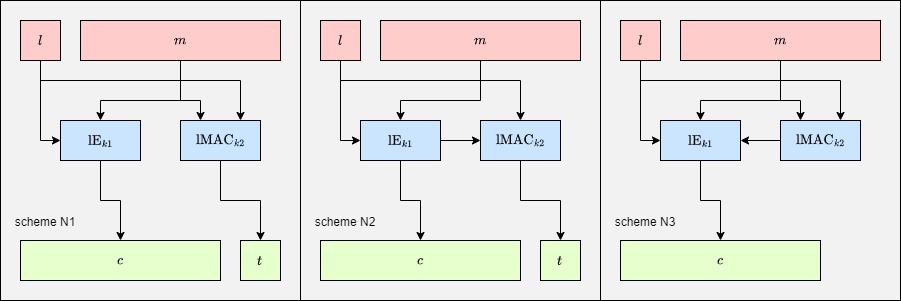
\includegraphics[scale = 0.4]{images/N-schemes.png}
\caption{Adjusted N schemes from \nrs}
\label{fig: N schemes}
\end{figure}

\begin{figure}
    \begin{pchstack}[boxed,center,space=0.5cm]
        \pseudocode[lnstart=-1,linenumbering,head={AE.enc$(\keyinstance,\lockinstance,\messageinstance)$}]{
            (\keyinstance{}1,\keyinstance{}2) \result \keyinstance \\
            \ciphertextinstance' \result \text{E.enc}(\keyinstance{}1,\lockinstance,\messageinstance) \\
            \taginstance \result \text{M.mac}(\keyinstance{}2,\lockinstance,\messageinstance) \\
            \ciphertextinstance \result (\ciphertextinstance',\taginstance)\\
            \pcreturn \ciphertextinstance
        }
        \pseudocode[lnstart=4,linenumbering,head={AE.dec$(\keyinstance,\lockinstance,\ciphertextinstance)$}]{
            (\keyinstance{}1,\keyinstance{}2) \result \keyinstance \\
            (\ciphertextinstance',\taginstance) \result \ciphertextinstance \\
            \messageinstance \result \text{E.dec}(\keyinstance{}1,\lockinstance,\ciphertextinstance') \\
            \taginstance' \result \text{M.mac}(\keyinstance{}2,\lockinstance,\messageinstance) \\
            \pcif \taginstance \neq \taginstance' : \messageinstance \result \invalid\\
            \pcreturn \messageinstance
        }
    \end{pchstack}
\caption{AE.enc an AE.dec based on N1}
\label{fig: N1 calls}
\end{figure}

\begin{figure}
    \begin{pchstack}[boxed,center,space=0.5cm]
        \pseudocode[lnstart=-1,linenumbering,head={AE.enc$(\keyinstance,\lockinstance,\messageinstance)$}]{
            (\keyinstance{}1,\keyinstance{}2) \result \keyinstance\\
            \ciphertextinstance' \result \text{E.enc}(\keyinstance{}1,\lockinstance,\messageinstance)\\
            \taginstance \result \text{M.mac}(\keyinstance{}2,\lockinstance,\ciphertextinstance')\\
            \ciphertextinstance \result (\ciphertextinstance',\taginstance)\\
            \pcreturn \ciphertextinstance
        }
        \pseudocode[lnstart=4,linenumbering,head={AE.dec$(\keyinstance,\lockinstance,\ciphertextinstance)$}]{
            (\keyinstance{}1,\keyinstance{}2) \result \keyinstance\\
            (\ciphertextinstance',\taginstance) \result \ciphertextinstance\\
            \messageinstance \result \text{E.dec}(\keyinstance{}1,\lockinstance,\ciphertextinstance')\\
            \taginstance' \result \text{M.mac}(\keyinstance{}2,\lockinstance,\ciphertextinstance')\\
            \pcif \taginstance \neq \taginstance' : \messageinstance \result \invalid\\
            \pcreturn \messageinstance
        }
    \end{pchstack}
\caption{AE.enc an AE.dec based on N2}
\label{fig: N2 calls}
\end{figure}

\begin{figure}
    \begin{pchstack}[boxed,center,space=0.5cm]
        \pseudocode[lnstart=-1,linenumbering,head={AE.enc$(\keyinstance,\lockinstance,\messageinstance)$}]{
            (\keyinstance{}1,\keyinstance{}2) \result \keyinstance\\
            \taginstance \result \text{M.mac}(\keyinstance{}2,\lockinstance,\messageinstance)\\
            \messageinstance' \result \messageinstance \concatinate \taginstance\\
            \ciphertextinstance \result \text{E.enc}(\keyinstance{}1,\lockinstance,\messageinstance')\\
            \pcreturn \ciphertextinstance
        }
        \pseudocode[lnstart=4,linenumbering,head={AE.dec$(\keyinstance,\lockinstance,\ciphertextinstance)$}]{
            (\keyinstance{}1,\keyinstance{}2) \result \keyinstance\\
            \messageinstance' \result \text{E.dec}(\keyinstance{}1,\lockinstance,\ciphertextinstance)\\
            (\messageinstance,\taginstance) \result \messageinstance'\\
            \taginstance' \result \text{M.mac}(\keyinstance{}2,\lockinstance,\messageinstance)\\
            \pcif \taginstance \neq \taginstance' : \messageinstance \result \invalid\\
            \pcreturn \messageinstance
        }
    \end{pchstack}
\caption{AE.enc an AE.dec based on N3}
\label{fig: N3 calls}
\end{figure}

\subsection{Security Bounds}
We define the composition secure if there is a tight reduction from breaking the lAE-security of the scheme to breaking the lE-security or the lMAC security of the underlying primitives. More specifically, we prove the following theorem:

\begin{theorem}
    Let lAE be constructed from lMAC and lE as described in Figure \ref{fig: N1 calls}, \ref{fig: N2 calls} or \ref{fig: N3 calls}. Let ciphertext space \ciphertextspace{} from the lE be a subset of message space \messagespace{} from the lMAC and let lMAC and lE have a shared lock space. Then, for any number of users \users{} and any lAE adversary \adversary{} that poses at most $Q_e$ many Oenc queries, and at most $Q_d$ many Odec queries, there exist a lMAC adversary $B$ and a lE adversary $C$ such that:
    \textnormal{
    \begin{align*}
        \text{\advantage{$A$,\users}{lAE}} \leq \text{\advantage{$B$,\users}{lMAC}} + \text{\advantage{$C$,\users}{lE}} + \frac{Q_d}{2^{\text{n}}},
    \end{align*}
    }
    where \textnormal{n} is the output length of the lMAC in bits. The running time of $B$ is at most that of A plus the time required to run $Q_e$ many \textnormal{E.enc} encapsulations and $Q_d$ many \textnormal{E.dec} decapsulations. The running time of $C$ is at most that of \adversary. Additionally, $B$ makes at most $Q_e$ many Omac queries and at most $Q_d$ many Ovrf queries and $C$ makes at most $Q_e$ many Oenc queries.
\end{theorem}
\noindent
Within this theorem, both $Q_e$ and $Q_d$ refer to the total queries the adversary is allowed to make, not the queries per user. As a result $Q_e$ is limited by \users.

\section{Security proof}
To prove theorem 1, we prove it separately for N1, N2 and N3. In this section, the full proof of case N1 can be found, as well as the main differences between the three cases. The full proof of case N2 and N3 can be found in appendix A.
\paragraph*{N1}
First, we repeat theorem 1 with N1 filled in:
\begin{theorem}
Let lAE be constructed from lMAC and lE as described in Figure \ref{fig: N1 calls}. Let ciphertext space \ciphertextspace{} from the lE be a subset of message space \messagespace{} from the lMAC and let lMAC and lE have a shared lock space. Then, for any number of users \users{} and any lAE adversary \adversary{} that poses at most $Q_e$ many Oenc queries, and at most $Q_d$ many Odec queries, there exist a lMAC adversary $B$ and a lE adversary $C$ such that:
\textnormal{
\begin{align*}
    \text{\advantage{$A$,\users}{lAE}} \leq \text{\advantage{$B$,\users}{lMAC}} + \text{\advantage{$C$,\users}{lE}} + \frac{Q_d}{2^{\text{n}}},
\end{align*}
}
where \textnormal{n} is the output length of the lMAC in bits. The running time of $B$ is at most that of A plus the time required to run $Q_e$ many \textnormal{E.enc} encapsulations and $Q_d$ many \textnormal{E.dec} decapsulations. The running time of $C$ is at most that of \adversary. Additionally, $B$ makes at most $Q_e$ many Omac queries and at most $Q_d$ many Ovrf queries and $C$ makes at most $Q_e$ many Oenc queries.
\end{theorem}
\noindent
Within this theorem, both $Q_e$ and $Q_d$ refer to the total queries the adversary is allowed to make, not the queries per user. As a result $Q_e$ is limited by \users.
\begin{proof}
To prove this theorem, we start by defining game lAE-N1 in Figure \ref{fig: lAE-N1 game}. This game is the game lAE-IND-\$-CCA (Figure \ref{fig: lAE-IND game}), with AE.enc and AE.dec substituted with the N1 algorithms from Figure \ref{fig: N1 calls}.
\begin{figure}[H]
    \begin{pchstack}[boxed,center,space=0.5cm]
        \pseudocode[lnstart=-1,linenumbering,head={\textbf{Game} lAE-N1$^{b}_{\adversary,\users}$ }]{
        L \result \emptyset\\
        \pcfor \user \in [1..N]:\\
        \t \keyinstance_\user \sample \keyspace\\
        \t C_\user \result \invalid\\
        b' \result \adversary\\
        \pcreturn b'
        }
        \pseudocode[lnstart=5,linenumbering,head={\textbf{Oracle} Oenc$(\user,\lockinstance,\messageinstance)$}]{
            \pcif C_\user \neq \invalid: \pcreturn \invalid\\
            \pcif \lockinstance \in L: \pcreturn \invalid\\
            L \result L \cup \{\lockinstance\}\\
            \lockinstance_\user \result \lockinstance\\
            (\keyinstance{}1,\keyinstance{}2) \result \keyinstance_j\\
            \ciphertextinstance' \result \text{E.enc}(\keyinstance{}1,\lockinstance_j,\messageinstance)\\
            \taginstance \result \text{M.mac}(\keyinstance{}2,\lockinstance_j,\messageinstance)\\
            \ciphertextinstance \result (\ciphertextinstance',\taginstance)\\
            \pcif b = 1 \wedge \ciphertextinstance \neq \invalid: \\
            \t \ciphertextinstance \sample \{0,1\}^{\abs{\ciphertextinstance}}\\
            C_\user \result \ciphertextinstance\\
            \pcreturn \ciphertextinstance
        }
        \pseudocode[lnstart=17,linenumbering,head={\textbf{Oracle} Odec$(\user,\ciphertextinstance)$}]{
            \pcif C_\user = \invalid: \pcreturn \invalid\\
            \pcif \ciphertextinstance = C_\user: \pcreturn \invalid\\
            (\keyinstance{}1,\keyinstance{}2) \result \keyinstance_j\\
            (\ciphertextinstance',\taginstance) \result \ciphertextinstance\\
            \messageinstance \result \text{E.dec}(\keyinstance{}1,\lockinstance_j,\ciphertextinstance')\\
            \taginstance' \result \text{M.mac}(\keyinstance{}2,\lockinstance_j,\messageinstance)\\
            \pcif \taginstance \neq \taginstance' : \messageinstance \result \invalid\\
            \pcif b = 1 : \messageinstance \result \invalid\\
            \pcreturn \messageinstance
        }
    \end{pchstack}
    \caption{lAE-N1 game, adversary{} has access to oracles Oenc and Odec.}
    \label{fig: lAE-N1 game}
\end{figure}

\noindent By definition, this gives us
\begin{align*}
    \text{\advantage{$A$,\users}{lAE}}
    =
    \text{Pr}[\text{lAE-N1}_{\text{\adversary,\users}}^0 =0]
    -
    \text{Pr}[\text{lAE-N1}_{\text{\adversary,\users}}^1 =0].
\end{align*}
Next we define game N1-switch-1 in Figure \ref{fig: N1-switch-1 game}. The only difference between this game and game lAE-N1$^0$ is the fact that N1-switch-1 uses the uniformly random function $tag$, instead of the lMAC. To define this function we write $\mathit{Func}(\keyspace \times \lockspace \times \messagespace,\tagspace)$ to denote the set of all functions from the key space of the MAC \keyspace, the shared lock space \lockspace{} and message space \messagespace{} to the tag space \tagspace. We define this function specifically as we want the tags resulting from computations in oracle Oenc to match with those in oracle Odec. When the input of $tag$ is outside its domain, it will return \invalid.

\begin{figure}[H]
    \begin{pchstack}[boxed,center,space=0.5cm]
        \pseudocode[lnstart=-1,linenumbering,head={\textbf{Game} N1-switch-1$_{\adversary,\users}$ }]{
        L \result \emptyset\\
        tag \sample \mathit{Func}(\keyspace_{mac}\times \lockspace \times \messagespace, \tagspace)\\
        \pcfor \user \in [1..N]:\\
        \t \keyinstance_\user \sample \keyspace\\
        \t C_\user \result \invalid\\
        b' \result \adversary\\
        \pcreturn b'
        }
        \pseudocode[lnstart=6,linenumbering,head={\textbf{Oracle} Oenc$(\user,\lockinstance,\messageinstance)$}]{
            \pcif C_\user \neq \invalid: \pcreturn \invalid\\
            \pcif \lockinstance \in L: \pcreturn \invalid\\
            L \result L \cup \{\lockinstance\}\\
            \lockinstance_\user \result \lockinstance\\
            (\keyinstance{}1,\keyinstance{}2) \result \keyinstance_j\\
            \ciphertextinstance' \result \text{E.enc}(\keyinstance{}1,\lockinstance_j,\messageinstance)\\
            \taginstance \result tag(\keyinstance{}2,\lockinstance_j,\messageinstance)\\
            \ciphertextinstance \result (\ciphertextinstance',\taginstance)\\
            C_\user \result \ciphertextinstance\\
            \pcreturn \ciphertextinstance
        }
        \pseudocode[lnstart=16,linenumbering,head={\textbf{Oracle} Odec$(\user,\ciphertextinstance)$}]{
            \pcif C_\user = \invalid: \pcreturn \invalid\\
            \pcif \ciphertextinstance = C_\user: \pcreturn \invalid\\
            (\keyinstance{}1,\keyinstance{}2) \result \keyinstance_j\\
            (\ciphertextinstance',\taginstance) \result \ciphertextinstance\\
            \messageinstance \result \text{E.dec}(\keyinstance{}1,\lockinstance_j,\ciphertextinstance')\\
            \taginstance' \result tag(\keyinstance{}2,\lockinstance_j,\messageinstance)\\
            \pcif \taginstance \neq \taginstance' : \messageinstance \result \invalid\\
            \pcreturn \messageinstance
        }
    \end{pchstack}
    \caption{N1-switch-1, adversary{} has access to oracles Oenc and Odec. 
    Key space $\keyspace_{mac}$ is the key space from M.mac. Lines 13 and 22 are different compared to lAE-N1$^0$, additionally lines 14, 15 and 25 from lAE-N1 are removed.}
    \label{fig: N1-switch-1 game}
\end{figure}

\noindent
Using this game, we expand the probability:
\begin{align*}
    \text{\advantage{$A$,\users}{lAE}}
    &=
    \text{Pr}[\text{lAE-N1}_{\text{\adversary,\users}}^0 =0]
    -
    \text{Pr}[\text{N1-switch-1}_{\text{\adversary,\users}} =0]
    \\&   + \text{Pr}[\text{N1-switch-1}_{\text{\adversary,\users}} =0]
    -
    \text{Pr}[\text{lAE-N1}_{\text{\adversary,\users}}^1 =0].
\end{align*}
Next, we can rewrite $\text{Pr}[\text{lAE-N1}_{\text{\adversary,\users}} =0] - \text{Pr}[\text{N1-switch-1}_{\text{\adversary,\users}} =0]$ into a lMAC advantage. To do so, we define adversary $B$ against lMAC in Figure \ref{fig: adversary B N1}. This adversary is playing game lMAC-PRF (Figure \ref{fig: lMAC-PRF game}), and has access to \adversary. 
\begin{figure}[H]
    \begin{pchstack}[boxed,center,space=0.5cm]
        \pseudocode[lnstart=-1,linenumbering,head={\textbf{Adverary} $B$}]{
        L \result \emptyset\\
        \pcfor \user \in [1..N]:\\
        \t \keyinstance_\user \sample \keyspace_{enc}\\
        \t C_\user \result \invalid\\
        b' \result \textbf{run } \adversary\\
        \pcreturn b'
        }
        \pseudocode[lnstart=5,linenumbering,head={\text{if \adversary{} calls }\textbf{Oracle} Oenc$(\user,\lockinstance,\messageinstance)$}]{
            \pcif C_\user \neq \invalid: \pcreturn \invalid\\
            \pcif \lockinstance \in L: \pcreturn \invalid\\
            L \result L \cup \{\lockinstance\}\\
            \lockinstance_\user \result \lockinstance\\
            \ciphertextinstance' \result \text{E.enc}(\keyinstance_j,\lockinstance_j,\messageinstance)\\
            \taginstance \result \text{Omac}(\user,\lockinstance_j,\messageinstance)\\
            \ciphertextinstance \result (\ciphertextinstance',\taginstance)\\
            C_\user \result \ciphertextinstance\\
            \pcreturn \ciphertextinstance
        }
        \pseudocode[lnstart=14,linenumbering,head={\text{if \adversary{} calls }\textbf{Oracle} Odec$(\user,\ciphertextinstance)$}]{
            \pcif C_\user = \invalid: \pcreturn \invalid\\
            \pcif \ciphertextinstance = C_\user: \pcreturn \invalid\\
            (\ciphertextinstance',\taginstance) \result \ciphertextinstance\\
            \messageinstance \result \text{E.dec}(\keyinstance{}_j,\lockinstance_j,\ciphertextinstance')\\
            passed \result \text{Ovrf}(\user,\messageinstance,\taginstance')\\
            \pcif \neg passed : \messageinstance \result \invalid\\
            \pcreturn \messageinstance
        }
    \end{pchstack}
    \caption{Adversary $B$, has access to \adversary{} and oracles Omac and Ovrf. Key space $\keyspace_{enc}$ is the key space from E.enc.}
    \label{fig: adversary B N1}
\end{figure}

\noindent
The runtime of $B$ is that of $A$. For every Oenc query \adversary{} makes, $B$ computes E.enc once, and calls Omac once. For every Odec query \adversary{} makes, $B$ computes E.dec once and calls Ovrf once. Note that, alternatively, $B$ could return 0 if $passed$ is \codetrue{} to avoid having to do E.dec computations. To increase consistency with the other two cases, these computations are still made. We can see that $\text{Pr}[\text{lMAC-PRF}_{\text{$B$,\users}}^0 =0]=\text{Pr}[\text{lAE-N1}_{\text{\adversary,\users}}^0 =0]$ as $B$ perfectly simulates game lAE-N1 with $b$ = 0 when its own $b$ is 0. In addition, $\text{Pr}[\text{lMAC-PRF}_{\text{$B$,\users}}^1 =0]=\text{Pr}[\text{N1-switch-1}_{\text{\adversary,\users}} =0]$ as $B$ perfectly simulates game N1-switch-1 whenever its own $b$ is 1. As a result, we can rewrite our advantage to:
\begin{align*}
    \text{\advantage{$A$,\users}{lAE}}
    &=
    \text{Pr}[\text{lAE-N1}_{\text{\adversary,\users}}^0 =0]
    -
    \text{Pr}[\text{N1-switch-1}_{\text{\adversary,\users}} =0]
    \\&  + \text{Pr}[\text{N1-switch-1}_{\text{\adversary,\users}} =0]
    -
    \text{Pr}[\text{lAE-N1}_{\text{\adversary,\users}}^1 =0]
    \\& =
    \text{Pr}[\text{lMAC-PRF}_{\text{$B$,\users}}^0 =0]
    -
    \text{Pr}[\text{lMAC-PRF}_{\text{$B$,\users}}^1 =0]
    \\&  + \text{Pr}[\text{N1-switch-1}_{\text{\adversary,\users}} =0]
    -
    \text{Pr}[\text{lAE-N1}_{\text{\adversary,\users}}^1 =0]
    \\& = \text{\advantage{$B$,\users}{lMAC}}
    + \text{Pr}[\text{N1-switch-1}_{\text{\adversary,\users}} =0]
    -
    \text{Pr}[\text{lAE-N1}_{\text{\adversary,\users}}^1 =0].
\end{align*}
To expand our advantage again, we define game N1-switch-2 in Figure \ref{fig: N1-switch-2 game}. Apart from the Odec query, this game is equivalent to the first switch game. The Odec oracle from N1-switch-2 always returns \invalid{}, it is written down more elaborately to include the event $bad$. This is added to event supports a well-known proof tactic \cite{EC:BelRog06}. Our expanded advantage is:
\begin{align*}
    \text{\advantage{$A$,\users}{lAE}}
    &=
    \text{\advantage{$B$,\users}{lMAC}} 
    +
    \text{Pr}[\text{N1-switch-1}_{\text{\adversary,\users}} =0]
    -
    \text{Pr}[\text{N1-switch-2}_{\text{\adversary,\users}} =0]
    \\& +
    \text{Pr}[\text{N1-switch-2}_{\text{\adversary,\users}} =0]
    -
    \text{Pr}[\text{lAE-N1}_{\text{\adversary,\users}}^1 =0].
\end{align*}
\begin{figure}[H]
    \begin{pchstack}[boxed,center,space=0.5cm]
        \pseudocode[lnstart=-1,linenumbering,head={\textbf{Game} N1-switch-2$_{\adversary,\users}$ }]{
        L \result \emptyset\\
        tag \sample \mathit{Func}(\keyspace_{mac}\times \lockspace \times \messagespace,\tagspace)\\
        \pcfor \user \in [1..N]:\\
        \t \keyinstance_\user \sample \keyspace\\
        \t C_\user \result \invalid\\
        b' \result \adversary\\
        \pcreturn b'
        }
        \pseudocode[lnstart=6,linenumbering,head={\textbf{Oracle} Oenc$(\user,\lockinstance,\messageinstance)$}]{
            \pcif C_\user \neq \invalid: \pcreturn \invalid\\
            \pcif \lockinstance \in L: \pcreturn \invalid\\
            L \result L \cup \{\lockinstance\}\\
            \lockinstance_\user \result \lockinstance\\
            (\keyinstance{}1,\keyinstance{}2) \result \keyinstance_j\\
            \ciphertextinstance' \result \text{E.enc}(\keyinstance{}1,\lockinstance_j,\messageinstance)\\
            \taginstance \result tag(\keyinstance{}2,\lockinstance_j,\messageinstance)\\
            \ciphertextinstance \result (\ciphertextinstance',\taginstance)\\
            C_\user \result \ciphertextinstance\\
            \pcreturn \ciphertextinstance
        }
        \pseudocode[lnstart=16,linenumbering,head={\textbf{Oracle} Odec$(\user,\ciphertextinstance)$}]{
            \pcif C_\user = \invalid: \pcreturn \invalid\\
            \pcif \ciphertextinstance = C_\user: \pcreturn \invalid\\
            (\keyinstance{}1,\keyinstance{}2) \result \keyinstance_j\\
            (\ciphertextinstance',\taginstance) \result \ciphertextinstance\\
            \messageinstance \result \text{E.dec}(\keyinstance{}1,\lockinstance_j,\ciphertextinstance')\\
            \taginstance' \result tag(\keyinstance{}2,\lockinstance_j,\messageinstance)\\
            \pcif \taginstance \neq \taginstance' : \messageinstance \result \invalid\\
            \pcelse: \\
            \t bad \result \codetrue\\
            \t \messageinstance \result \invalid\\
            \pcreturn \messageinstance
        }
    \end{pchstack}
    \caption{N1-switch-2 game, adversary{} has access to oracles Oenc and Odec. Key space $\keyspace_{mac}$ is the key space from M.mac. Line 24-26 are different compared to N1-switch-1.}
    \label{fig: N1-switch-2 game}
\end{figure}
\noindent
As N1-switch-1 and N1-switch-2 are so called identical-until-$bad$ \cite{EC:BelRog06}, meaning they are equivalent as long as the event $bad$ is not set to \codetrue, we know:
\begin{align*}
    \text{Pr}[\text{N1-switch-1}_{\text{\adversary,\users}} =0]-\text{Pr}[\text{N1-switch-2}_{\text{\adversary,\users}} =0] \leq \text{Pr}[bad=\codetrue].
\end{align*}
As $bad$ is set to \codetrue{} if, and only if, \taginstance=\taginstance$'$, we can state $\text{Pr}[bad=\codetrue] = \text{Pr}[\taginstance=\taginstance']$. The adversary needs to provide tag \taginstance{} and ciphertext \ciphertextinstance$'$, where ciphertext \ciphertextinstance$'$ leads to a message \messageinstance{} that is used as input to the $tag$ function. The provided tag-ciphertext pair may not be the result of the encryption query corresponding to the provided user. Combined with the tidiness of the encryption, it is ensured that, for any sensible adversarial query, the message \messageinstance{} cannot be the message which is encrypted for the provided user. This is because if \messageinstance{} would be the encrypted message, the correct tag cannot be provided and thus no information can be gained with the query. Consequently, \taginstance{} and \taginstance$'$ are only equal when the adversary is able to guess the output of $tag$ for a message that is not encrypted for the provided user. The function $tag$ is uniformly random so, with every fresh ciphertext, the probability that \taginstance{} and \taginstance$'$ are equal is $\frac{1}{2^{\text{n}}}$. Combined with at most $Q_d$ Odec queries we get $\text{Pr}[\taginstance=\taginstance'] = \text{Pr}[bad=\codetrue] \leq \frac{Q_d}{2^{\text{n}}}$ and thus, we can fill in $\text{Pr}[\text{N2-switch-1}_{\text{\adversary,\users}} =0]-\text{Pr}[\text{N1-switch-2}_{\text{\adversary,\users}} =0] \leq \text{Pr}[bad=\codetrue] \leq \frac{Q_d}{2^{\text{n}}}$ to obtain:
\begin{align*}
    \text{\advantage{$A$,\users}{lAE}}
    &\leq
    \text{\advantage{$B$,\users}{lMAC}} 
    +
    \text{Pr}[\text{N1-switch-2}_{\text{\adversary,\users}} =0]
    -
    \text{Pr}[\text{lAE-N2}_{\text{\adversary,\users}}^1 =0].
    +
    \frac{Q_d}{2^{\text{n}}}
\end{align*}
We define game N1-switch-3 in Figure \ref{fig: N1-switch-3 game} to expand our advantage one last time. Switch game 3 is equivalent to switch game 2 but always returns lazily sampled random bits when the outcome of E.enc is valid. It might seem like there is a difference as \taginstance can no longer become \invalid. This is not the case as, due to the chosen input spaces of tag, tag can only return \invalid{} whenever \ciphertextinstance$'$ is already \invalid. As a result, tag will never influence wether or not \ciphertextinstance{} on line 12 is \invalid. We also simplify Odec as we no longer need the event $bad$. We use this game to expand our advantage to:
\begin{align*}
    \text{\advantage{$A$,\users}{lAE}}
    &\leq
    \text{\advantage{$B$,\users}{lMAC}} 
    +
    \text{Pr}[\text{N1-switch-2}_{\text{\adversary,\users}} =0]
    -
    \text{Pr}[\text{N1-switch-3}_{\text{\adversary,\users}} =0]
    \\& +
    \text{Pr}[\text{N1-switch-3}_{\text{\adversary,\users}} =0]
    -
    \text{Pr}[\text{lAE-N1}_{\text{\adversary,\users}}^1 =0].
    +
    \frac{Q_d}{2^{\text{n}}}
\end{align*}

\begin{figure}[H]
    \begin{pchstack}[boxed,center,space=0.5cm]
        \pseudocode[lnstart=-1,linenumbering,head={\textbf{Game} N1-switch-3$_{\adversary,\users}$ }]{
        L \result \emptyset\\
        \pcfor \user \in [1..N]:\\
        \t \keyinstance_\user \sample \keyspace_{enc}\\
        \t C_\user \result \invalid\\
        b' \result \adversary\\
        \pcreturn b'
        }
        \pseudocode[lnstart=5,linenumbering,head={\textbf{Oracle} Oenc$(\user,\lockinstance,\messageinstance)$}]{
            \pcif C_\user \neq \invalid: \pcreturn \invalid\\
            \pcif \lockinstance \in L: \pcreturn \invalid\\
            L \result L \cup \{\lockinstance\}\\
            \lockinstance_\user \result \lockinstance\\
            \ciphertextinstance' \result \text{E.enc}(\keyinstance{}j,\lockinstance_j,\messageinstance)\\
            \taginstance \sample \{0,1\}^{\text{n}}\\
            \ciphertextinstance \result (\ciphertextinstance',\taginstance)\\
            \pcif \ciphertextinstance \neq \invalid: \\
            \t \ciphertextinstance \sample \{0,1\}^{\abs{\ciphertextinstance}}\\
            C_\user \result \ciphertextinstance\\
            \pcreturn \ciphertextinstance
        }
        \pseudocode[lnstart=17,linenumbering,head={\textbf{Oracle} Odec$(\user,\ciphertextinstance)$}]{
            \pcreturn \invalid
        }
    \end{pchstack}
    \caption{N1-switch-3 game, adversary{} has access to oracles Oenc and Odec. Key space $\keyspace_{enc}$ is the key space from E.enc. Line 14 and 15 are different compared to N1-switch-2, and Odec is simplified.}
    \label{fig: N1-switch-3 game}
\end{figure}
\noindent
$\text{Pr}[\text{N1-switch-3}_{\text{\adversary,\users}} =0]$ and $\text{Pr}[\text{lAE-N1}_{\text{\adversary,\users}}^1 =0]$ are equivalent by definition, giving:
\begin{align*}
    \text{\advantage{$A$,\users}{lAE}}
    &\leq
    \text{\advantage{$B$,\users}{lMAC}} 
    +
    \text{Pr}[\text{N1-switch-2}_{\text{\adversary,\users}} =0]
    -
    \text{Pr}[\text{N1-switch-3}_{\text{\adversary,\users}} =0]
    +
    \frac{Q_d}{2^{\text{n}}}
\end{align*}
Next, we can rewrite $\text{Pr}[\text{N1-switch-2}_{\text{\adversary,\users}} =0] - \text{Pr}[\text{N1-switch-3}_{\text{\adversary,\users}} =0]$ into a lE advantage. To do so, we define adversary $C$ against lE in Figure \ref{fig: adversary c N1}. This adversary is playing game lE-IND-\$-CPA (Figure \ref{fig: lE-IND game}), and has access to \adversary. 
\begin{figure}[H]
    \begin{pchstack}[boxed,center,space=0.5cm]
        \pseudocode[lnstart=-1,linenumbering,head={\textbf{Adverary} $C$}]{
        L \result \emptyset\\
        \pcfor \user \in [1..N]:\\
        \t C_\user \result \invalid\\
        b' \result \textbf{run } \adversary\\
        \pcreturn b'
        }
        \pseudocode[lnstart=4,linenumbering,head={\text{if \adversary{} calls }\textbf{Oracle} Oenc$(\user,\lockinstance,\messageinstance)$}]{
            \pcif C_\user \neq \invalid: \pcreturn \invalid\\
            \pcif \lockinstance \in L: \pcreturn \invalid\\
            L \result L \cup \{\lockinstance\}\\
            \lockinstance_\user \result \lockinstance\\
            \ciphertextinstance' \result \text{Oenc}(\user,\lockinstance_j,\messageinstance)\\
            \taginstance \sample \{0,1\}^{\text{n}}\\
            \ciphertextinstance \result (\ciphertextinstance',\taginstance)\\
            C_\user \result \ciphertextinstance\\
            \pcreturn \ciphertextinstance
        }
        \pseudocode[lnstart=13,linenumbering,head={\text{if \adversary{} calls }\textbf{Oracle} Odec$(\user,\ciphertextinstance)$}]{
            \pcreturn \invalid
        }
    \end{pchstack}
    \caption{Adversary $C$, has access to \adversary{} and oracle Oenc. Note the Oenc in line 9 refers to the encryption oracle Oenc that $C$ has access to, not the oracle Oenc $A$ has access to.}
    \label{fig: adversary c N1}
\end{figure}
\noindent
The runtime of $C$ is that of $A$. For every Oenc query $A$ makes, $C$ makes one Oenc query. We can see that $\text{Pr}[\text{N1-switch-2}_{\text{\adversary,\users}} =0] = \text{Pr}[\text{lE-IND-\$-CPA}_{\text{$C$,\users}}^0 =0]$ as $C$ perfectly simulates N1-switch-2 when its own $b$ is 0. When its own $b$ is 1, $C$ perfectly simulates N1-switch-3 giving $\text{Pr}[\text{N1-switch-3}_{\text{\adversary,\users}} =0] = \text{Pr}[\text{lE-IND-\$-CPA}_{\text{$C$,\users}}^1 =0]$. This leads us to:
\begin{align*}
    \text{\advantage{$A$,\users}{lAE}}
    &\leq
    \text{\advantage{$B$,\users}{lMAC}} 
    +
    \text{Pr}[\text{N1-switch-2}_{\text{\adversary,\users}} =0]
    -
    \text{Pr}[\text{N1-switch-3}_{\text{\adversary,\users}} =0]
    +
    \frac{Q_d}{2^{\text{n}}}.
    \\& \leq
    \text{\advantage{$B$,\users}{lMAC}} 
    +
    \text{Pr}[\text{lE-IND-\$-CPA}_{\text{$C$,\users}}^0 =0]
    -
    \text{Pr}[\text{lE-IND-\$-CPA}_{\text{$C$,\users}}^1 =0]
    +
    \frac{Q_d}{2^{\text{n}}}.
    \\& \leq
    \text{\advantage{$B$,\users}{lMAC}} 
    +
    \text{\advantage{$C$,\users}{lE}}
    +
    \frac{Q_d}{2^{\text{n}}}
\end{align*}
Thus Proving:
\begin{align*}
    \text{\advantage{$A$,\users}{lAE}}
    \leq
    \text{\advantage{$B$,\users}{lMAC}} 
    +
    \text{\advantage{$C$,\users}{lE}}
    +
    \frac{Q_d}{2^{\text{n}}}
\end{align*}
\end{proof}
\paragraph*{N2 and N3}
Structurally, the three proofs are identical. For each case, the games, as well as the adversaries, are adjusted to AE.enc and AE.dec corresponding to the N-scheme. As a result, they differ in the three lines generating \ciphertextinstance{} and the three lines generating \taginstance'. As a example the games lAE-N1 in figure \ref*{fig: lAE-N1 game}, lAE-N2 in figure \ref*{fig: lAE-N2 game} and lAE-N3 in figure \ref*{fig: lAE-N3 game} only differ on lines 11 to 13 and lines 21 to 23. In addition the input spaces to the functions are different to facilitate this change. The argument leading to $\text{Pr}[bad=\codetrue] \leq \frac{Q_d}{2^{\text{n}}}$ is different for the three cases as the tags are generated in a different way. To highlight this difference, the argument is put in between horizontal bars in the proof for N2 and N3. \textbf{(question: is this enough explanation and is it okay to highlight it with horizontal bars?)}
\section{Use Cases}
.
\subsection{PKE Schemes}
.
\subsection{MLS?}
.
\subsection{Secure channels?}
.
\section{Related Work} \label{sec: related work}
The idea of "locks", used for our lAE, originates from GKP, where augmentation with locks is proposed as an alternative to key expansion in a multi user setting in order to prevent ephemeral key collisions between users. They show how ephemeral key collisions can lead to insecurities, as well as how you can augment security primitives with locks. Afterwards, a composition of an augmented MAC and an augmented DEM is shown be suitable for hybrid encryption.
\\\\
The generic composition of authenticated encryption was first studied by Bellare and Namprempre \cite{AC:BelNam00}. The three most common composition modes encrypt-and-MAC, encrypt-then-MAC and MAC-then-encrypt are introduced and evaluated using a probabilistic encryption block. They find generic construction to be secure when using the encrypt-then-MAC method. NRS further investigate these modes of composition and state that the type of encryption primitive used, as well as the required end-result, influences which compositions are secure. They investigate ways to compose a nonce-based authenticated encryption scheme. Using IV-based encryption, 8 schemes are proven secure. Using nonce-based encryption 3 schemes, relating to encrypt-and-MAC, encrypt-then-MAC and MAC-then-encrypt, are proven secure.
\\\\
As an alternative to generic composition, authenticated encryption can also be composed non-generically. In this fashion, Rogaway, Bellare and Black propose OCB as a non-generic authenticated encryption construction \cite{CCS:RBBK01}. OCB is highly parallelizable and is cheaper in computation compared to generic construction. In the basic form, it can not take in associated data but an extension has been given to allow for this. It is proven secure whenever the underlying block cipher is secure. McGrew and Viega propose Galois/Counter Mode, GCM as a non-generic authenticated encryption construction \cite{mcgrew2004security}. Is a highly efficient mode of operation, also due to its parallelizability. It incorporates counter mode using a even length block cipher and supports the usage of associated data. In a addition to authenticated encryption, it can also be used as a standalone MAC function. Other non-generic modes of operation exist as well, but these two are the most popular.

\section{Open Problems}
In this section, we will look at some related challenges that are left unsolved. Wherever possible we will also indicate what needs to be done in order to solve these problems.

\paragraph*{Other N schemes}
NRS finds 20 possible N-schemes, of which 3 are proven secure. In this thesis, the only N-schemes evaluated are alterations on the ones proven secure by NRS. To more thoroughly investigate the security of generic lAE compositions, the other N-schemes should also be proven secure or be proven insecure with a counterexample. The amount of possible generic compositions gets bigger if the authenticated encryption scheme has more inputs. Without incorporating AD, only 10 out of 20 possible N-schemes remain. Three of these schemes are proven secure in this work, leaving 7 schemes to be evaluated.

\paragraph*{Adding associated Data}
The lAE construction is only evaluated without associated data (AD). To incorporate AD, a slight modification should be made to the definition of the lAE. With AD added, there will be 20 possible N-schemes, three of which will relate to the secure schemes from NRS. These three schemes should be prioritized as they have the highest likelihood of being secure. For a more rigorous analysis, all 20 schemes should be evaluated.

\paragraph*{Evaluating lAE with multiple uses}
The evaluation of the lAE construction is limited to a key that is used once. A more in-depth analysis could evaluate the construction in a setting where a key can be used multiple times. In order to maintain security, you would likely need to alter the lAE definition to also incorporate nonces. As the scheme will then have an additional input, a new set of possible compositions should be generated and evaluated. 

\paragraph*{Augmenting non-generic constructions with locks}
The non-generic constructions mentioned in section \ref{sec: related work} can possibly be augmented with locks as well. The augmented versions will most likely have lower computational cost when compared to generic composition, as well as be highly parallelizable. When proven secure, this will lead to more efficient instantiations of the lAE.

\section{Conclusion}

\newpage
\printbibliography[heading=bibintoc,title={References}]

\appendix
\section{Proof of N2 and N3}
In this appendix, the full proof of case N2 and N3 can be found.
\paragraph{N2}
First, we repeat theorem 1 with N2 filled in:
\begin{theorem}
Let lAE be constructed from lMAC and lE as described in Figure \ref{fig: N2 calls}. Let ciphertext space \ciphertextspace{} from the lE be a subset of message space \messagespace{} from the lMAC and let lMAC and lE have a shared lock space. Then, for any number of users \users{} and any lAE adversary \adversary{} that poses at most $Q_e$ many Oenc queries, and at most $Q_d$ many Odec queries, there exist a lMAC adversary $B$ and a lE adversary $C$ such that:
\textnormal{
\begin{align*}
    \text{\advantage{$A$,\users}{lAE}} \leq \text{\advantage{$B$,\users}{lMAC}} + \text{\advantage{$C$,\users}{lE}} + \frac{Q_d}{2^{\text{n}}},
\end{align*}}
where \textnormal{n} is the output length of the lMAC in bits. The running time of $B$ is at most that of A plus the time required to run $Q_e$ many \textnormal{E.enc} encapsulations and $Q_d$ many \textnormal{E.dec} decapsulations. The running time of $C$ is at most that of \adversary. Additionally, $B$ makes at most $Q_e$ many Omac queries and at most $Q_d$ many Ovrf queries and $C$ makes at most $Q_e$ many Oenc queries.
\end{theorem}
\noindent
Within this theorem, both $Q_e$ and $Q_d$ refer to the total queries the adversary is allowed to make, not the queries per user. As a result $Q_e$ is limited by \users.
\begin{proof}
To prove this theorem, we start by defining game lAE-N2 in Figure \ref{fig: lAE-N2 game}. This game is the game lAE-IND-\$-CCA (Figure \ref{fig: lAE-IND game}), with AE.enc and AE.dec substituted with the N2 algorithms from Figure \ref{fig: N2 calls}.
\begin{figure}[H]
    \begin{pchstack}[boxed,center,space=0.5cm]
        \pseudocode[lnstart=-1,linenumbering,head={\textbf{Game} lAE-N2$^{b}_{\adversary,\users}$ }]{
        L \result \emptyset\\
        \pcfor \user \in [1..N]:\\
        \t \keyinstance_\user \sample \keyspace\\
        \t C_\user \result \invalid\\
        b' \result \adversary\\
        \pcreturn b'
        }
        \pseudocode[lnstart=5,linenumbering,head={\textbf{Oracle} Oenc$(\user,\lockinstance,\messageinstance)$}]{
            \pcif C_\user \neq \invalid: \pcreturn \invalid\\
            \pcif \lockinstance \in L: \pcreturn \invalid\\
            L \result L \cup \{\lockinstance\}\\
            \lockinstance_\user \result \lockinstance\\
            (\keyinstance{}1,\keyinstance{}2) \result \keyinstance_j\\
            \ciphertextinstance' \result \text{E.enc}(\keyinstance{}1,\lockinstance_j,\messageinstance)\\
            \taginstance \result \text{M.mac}(\keyinstance{}2,\lockinstance_j,\ciphertextinstance')\\
            \ciphertextinstance \result (\ciphertextinstance',\taginstance)\\
            \pcif b = 1 \wedge \ciphertextinstance \neq \invalid: \\
            \t \ciphertextinstance \sample \{0,1\}^{\abs{\ciphertextinstance}}\\
            C_\user \result \ciphertextinstance\\
            \pcreturn \ciphertextinstance
        }
        \pseudocode[lnstart=17,linenumbering,head={\textbf{Oracle} Odec$(\user,\ciphertextinstance)$}]{
            \pcif C_\user = \invalid: \pcreturn \invalid\\
            \pcif \ciphertextinstance = C_\user: \pcreturn \invalid\\
            (\keyinstance{}1,\keyinstance{}2) \result \keyinstance_j\\
            (\ciphertextinstance',\taginstance) \result \ciphertextinstance\\
            \messageinstance \result \text{E.dec}(\keyinstance{}1,\lockinstance_j,\ciphertextinstance')\\
            \taginstance' \result \text{M.mac}(\keyinstance{}2,\lockinstance_j,\ciphertextinstance')\\
            \pcif \taginstance \neq \taginstance' : \messageinstance \result \invalid\\
            \pcif b = 1 : \messageinstance \result \invalid\\
            \pcreturn \messageinstance
        }
    \end{pchstack}
    \caption{lAE-N2 game, adversary{} has access to oracles Oenc and Odec.}
    \label{fig: lAE-N2 game}
\end{figure}

\noindent By definition, this gives us
\begin{align*}
    \text{\advantage{$A$,\users}{lAE}}
    =
    \text{Pr}[\text{lAE-N2}_{\text{\adversary,\users}}^0 =0]
    -
    \text{Pr}[\text{lAE-N2}_{\text{\adversary,\users}}^1 =0].
\end{align*}
Next we define game N2-switch-1 in Figure \ref{fig: N2-switch-1 game}. The only difference between this game and game lAE-N2$^0$ is the fact that N2-switch-1 uses the uniformly random function $tag$, instead of the lMAC. To define this function we write $\mathit{Func}(\keyspace \times \lockspace \times \ciphertextspace,\tagspace)$ to denote the set of all functions from the key space of the MAC \keyspace, the shared lock space \lockspace{} and ciphertext space from E.enc \ciphertextspace{} to the tag space \tagspace. We define this function specifically as we want the tags resulting from computations in oracle Oenc to match with those in oracle Odec. When the input of $tag$ is outside its domain, it will return \invalid.

\begin{figure}[H]
    \begin{pchstack}[boxed,center,space=0.5cm]
        \pseudocode[lnstart=-1,linenumbering,head={\textbf{Game} N2-switch-1$_{\adversary,\users}$ }]{
        L \result \emptyset\\
        tag \sample \mathit{Func}(\keyspace_{mac}\times \lockspace \times \ciphertextspace,\tagspace)\\
        \pcfor \user \in [1..N]:\\
        \t \keyinstance_\user \sample \keyspace\\
        \t C_\user \result \invalid\\
        b' \result \adversary\\
        \pcreturn b'
        }
        \pseudocode[lnstart=6,linenumbering,head={\textbf{Oracle} Oenc$(\user,\lockinstance,\messageinstance)$}]{
            \pcif C_\user \neq \invalid: \pcreturn \invalid\\
            \pcif \lockinstance \in L: \pcreturn \invalid\\
            L \result L \cup \{\lockinstance\}\\
            \lockinstance_\user \result \lockinstance\\
            (\keyinstance{}1,\keyinstance{}2) \result \keyinstance_j\\
            \ciphertextinstance' \result \text{E.enc}(\keyinstance{}1,\lockinstance_j,\messageinstance)\\
            \taginstance \result tag(\keyinstance{}2,\lockinstance_j,\ciphertextinstance')\\
            \ciphertextinstance \result (\ciphertextinstance',\taginstance)\\
            C_\user \result \ciphertextinstance\\
            \pcreturn \ciphertextinstance
        }
        \pseudocode[lnstart=16,linenumbering,head={\textbf{Oracle} Odec$(\user,\ciphertextinstance)$}]{
            \pcif C_\user = \invalid: \pcreturn \invalid\\
            \pcif \ciphertextinstance = C_\user: \pcreturn \invalid\\
            (\keyinstance{}1,\keyinstance{}2) \result \keyinstance_j\\
            (\ciphertextinstance',\taginstance) \result \ciphertextinstance\\
            \messageinstance \result \text{E.dec}(\keyinstance{}1,\lockinstance_j,\ciphertextinstance')\\
            \taginstance' \result tag(\keyinstance{}2,\lockinstance_j,\ciphertextinstance')\\
            \pcif \taginstance \neq \taginstance' : \messageinstance \result \invalid\\
            \pcreturn \messageinstance
        }
    \end{pchstack}
    \caption{N2-switch-1, adversary{} has access to oracles Oenc and Odec. 
    Key space $\keyspace_{mac}$ is the key space from M.mac. Lines 13 and 22 are different compared to lAE-N2$^0$, additionally lines 14, 15 and 25 from lAE-N2 are removed.}
    \label{fig: N2-switch-1 game}
\end{figure}

\noindent
Using this game, we expand the probability:
\begin{align*}
    \text{\advantage{$A$,\users}{lAE}}
    &=
    \text{Pr}[\text{lAE-N2}_{\text{\adversary,\users}}^0 =0]
    -
    \text{Pr}[\text{N2-switch-1}_{\text{\adversary,\users}} =0]
    \\&   + \text{Pr}[\text{N2-switch-1}_{\text{\adversary,\users}} =0]
    -
    \text{Pr}[\text{lAE-N2}_{\text{\adversary,\users}}^1 =0].
\end{align*}
Next, we can rewrite $\text{Pr}[\text{lAE-N2}_{\text{\adversary,\users}} =0] - \text{Pr}[\text{N2-switch-1}_{\text{\adversary,\users}} =0]$ into a lMAC advantage. To do so, we define adversary $B$ against lMAC in Figure \ref{fig: adversary B N2}. This adversary is playing game lMAC-PRF (Figure \ref{fig: lMAC-PRF game}), and has access to \adversary. 
\begin{figure}[H]
    \begin{pchstack}[boxed,center,space=0.5cm]
        \pseudocode[lnstart=-1,linenumbering,head={\textbf{Adverary} $B$}]{
        L \result \emptyset\\
        \pcfor \user \in [1..N]:\\
        \t \keyinstance_\user \sample \keyspace_{enc}\\
        \t C_\user \result \invalid\\
        b' \result \textbf{run } \adversary\\
        \pcreturn b'
        }
        \pseudocode[lnstart=5,linenumbering,head={\text{if \adversary{} calls }\textbf{Oracle} Oenc$(\user,\lockinstance,\messageinstance)$}]{
            \pcif C_\user \neq \invalid: \pcreturn \invalid\\
            \pcif \lockinstance \in L: \pcreturn \invalid\\
            L \result L \cup \{\lockinstance\}\\
            \lockinstance_\user \result \lockinstance\\
            \ciphertextinstance' \result \text{E.enc}(\keyinstance_j,\lockinstance_j,\messageinstance)\\
            \taginstance \result \text{Omac}(\user,\lockinstance_j,\ciphertextinstance')\\
            \ciphertextinstance \result (\ciphertextinstance',\taginstance)\\
            C_\user \result \ciphertextinstance\\
            \pcreturn \ciphertextinstance
        }
        \pseudocode[lnstart=14,linenumbering,head={\text{if \adversary{} calls }\textbf{Oracle} Odec$(\user,\ciphertextinstance)$}]{
            \pcif C_\user = \invalid: \pcreturn \invalid\\
            \pcif \ciphertextinstance = C_\user: \pcreturn \invalid\\
            (\ciphertextinstance',\taginstance) \result \ciphertextinstance\\
            \messageinstance \result \text{E.dec}(\keyinstance{}_j,\lockinstance_j,\ciphertextinstance')\\
            passed \result \text{Ovrf}(\user,\ciphertextinstance',\taginstance')\\
            \pcif \neg passed : \messageinstance \result \invalid\\
            \pcreturn \messageinstance
        }
    \end{pchstack}
    \caption{Adversary $B$, has access to \adversary{} and oracles Omac and Ovrf. Key space $\keyspace_{enc}$ is the key space from E.enc.}
    \label{fig: adversary B N2}
\end{figure}

\noindent
The runtime of $B$ is that of $A$. For every Oenc query \adversary{} makes, $B$ computes E.enc once, and calls Omac once. For every Odec query \adversary{} makes, $B$ computes E.dec once and calls Ovrf once. Note that, alternatively, $B$ could return 0 if $passed$ is \codetrue{} to avoid having to do E.dec computations. To increase consistency with the other two cases, these computations are still made. We can see that $\text{Pr}[\text{lMAC-PRF}_{\text{$B$,\users}}^0 =0]=\text{Pr}[\text{lAE-N2}_{\text{\adversary,\users}}^0 =0]$ as $B$ perfectly simulates game lAE-N2 with $b$ = 0 when its own $b$ is 0. In addition, $\text{Pr}[\text{lMAC-PRF}_{\text{$B$,\users}}^1 =0]=\text{Pr}[\text{N2-switch-1}_{\text{\adversary,\users}} =0]$ as $B$ perfectly simulates game N2-switch-1 whenever its own $b$ is 1. As a result, we can rewrite our advantage to:
\begin{align*}
    \text{\advantage{$A$,\users}{lAE}}
    &=
    \text{Pr}[\text{lAE-N2}_{\text{\adversary,\users}}^0 =0]
    -
    \text{Pr}[\text{N2-switch-1}_{\text{\adversary,\users}} =0]
    \\&  + \text{Pr}[\text{N2-switch-1}_{\text{\adversary,\users}} =0]
    -
    \text{Pr}[\text{lAE-N2}_{\text{\adversary,\users}}^1 =0]
    \\& =
    \text{Pr}[\text{lMAC-PRF}_{\text{$B$,\users}}^0 =0]
    -
    \text{Pr}[\text{lMAC-PRF}_{\text{$B$,\users}}^1 =0]
    \\&          + \text{Pr}[\text{N2-switch-1}_{\text{\adversary,\users}} =0]
    -
    \text{Pr}[\text{lAE-N2}_{\text{\adversary,\users}}^1 =0]
    \\& = \text{\advantage{$B$,\users}{lMAC}}
    + \text{Pr}[\text{N2-switch-1}_{\text{\adversary,\users}} =0]
    -
    \text{Pr}[\text{lAE-N2}_{\text{\adversary,\users}}^1 =0].
\end{align*}
To expand our advantage again, we define game N2-switch-2 in Figure \ref{fig: N2-switch-2 game}. Apart from the Odec query, this game is equivalent to the first switch game. The Odec oracle from N2-switch-2 always returns \invalid{}, it is written down more elaborately to include the event $bad$. This is added to event supports a well-known proof tactic \cite{EC:BelRog06}. Our expanded advantage is:
\begin{align*}
    \text{\advantage{$A$,\users}{lAE}}
    &=
    \text{\advantage{$B$,\users}{lMAC}} 
    +
    \text{Pr}[\text{N2-switch-1}_{\text{\adversary,\users}} =0]
    -
    \text{Pr}[\text{N2-switch-2}_{\text{\adversary,\users}} =0]
    \\& +
    \text{Pr}[\text{N2-switch-2}_{\text{\adversary,\users}} =0]
    -
    \text{Pr}[\text{lAE-N2}_{\text{\adversary,\users}}^1 =0].
\end{align*}
\begin{figure}[H]
    \begin{pchstack}[boxed,center,space=0.5cm]
        \pseudocode[lnstart=-1,linenumbering,head={\textbf{Game} N2-switch-2$_{\adversary,\users}$ }]{
        L \result \emptyset\\
        tag \sample \mathit{Func}(\keyspace_{mac}\times \lockspace \times \ciphertextspace,\tagspace)\\
        \pcfor \user \in [1..N]:\\
        \t \keyinstance_\user \sample \keyspace\\
        \t C_\user \result \invalid\\
        b' \result \adversary\\
        \pcreturn b'
        }
        \pseudocode[lnstart=6,linenumbering,head={\textbf{Oracle} Oenc$(\user,\lockinstance,\messageinstance)$}]{
            \pcif C_\user \neq \invalid: \pcreturn \invalid\\
            \pcif \lockinstance \in L: \pcreturn \invalid\\
            L \result L \cup \{\lockinstance\}\\
            \lockinstance_\user \result \lockinstance\\
            (\keyinstance{}1,\keyinstance{}2) \result \keyinstance_j\\
            \ciphertextinstance' \result \text{E.enc}(\keyinstance{}1,\lockinstance_j,\messageinstance)\\
            \taginstance \result tag(\keyinstance{}2,\lockinstance_j,\ciphertextinstance')\\
            \ciphertextinstance \result (\ciphertextinstance',\taginstance)\\
            C_\user \result \ciphertextinstance\\
            \pcreturn \ciphertextinstance
        }
        \pseudocode[lnstart=16,linenumbering,head={\textbf{Oracle} Odec$(\user,\ciphertextinstance)$}]{
            \pcif C_\user = \invalid: \pcreturn \invalid\\
            \pcif \ciphertextinstance = C_\user: \pcreturn \invalid\\
            (\keyinstance{}1,\keyinstance{}2) \result \keyinstance_j\\
            (\ciphertextinstance',\taginstance) \result \ciphertextinstance\\
            \messageinstance \result \text{E.dec}(\keyinstance{}1,\lockinstance_j,\ciphertextinstance')\\
            \taginstance' \result tag(\keyinstance{}2,\lockinstance_j,\ciphertextinstance')\\
            \pcif \taginstance \neq \taginstance' : \messageinstance \result \invalid\\
            \pcelse: \\
            \t bad \result \codetrue\\
            \t \messageinstance \result \invalid\\
            \pcreturn \messageinstance
        }
    \end{pchstack}
    \caption{N2-switch-2 game, adversary{} has access to oracles Oenc and Odec. Key space $\keyspace_{mac}$ is the key space from M.mac. Line 24-26 are different compared to N2-switch-1.}
    \label{fig: N2-switch-2 game}
\end{figure}
\noindent
As N2-switch-1 and N2-switch-2 are so called identical-until-$bad$ \cite{EC:BelRog06}, meaning they are equivalent as long as the event $bad$ is not set to \codetrue, we know:
\begin{align*}
    \text{Pr}[\text{N2-switch-1}_{\text{\adversary,\users}} =0]-\text{Pr}[\text{N2-switch-2}_{\text{\adversary,\users}} =0] \leq \text{Pr}[bad=\codetrue].
\end{align*}
\rule{5.8in}{1pt}\vspace{0,12cm}\\
As $bad$ is set to \codetrue{} if, and only if, \taginstance=\taginstance$'$, we can state $\text{Pr}[bad=\codetrue] = \text{Pr}[\taginstance=\taginstance']$. The adversary needs to provide tag \taginstance{} and ciphertext \ciphertextinstance$'$ for the $tag$ function, where the provided tag-ciphertext pair may not be the result of the encryption query corresponding to the provided user. Consequently, \taginstance{} and \taginstance$'$ are only equal when the adversary is able to guess the output of $tag$ for a ciphertext that is not encrypted for the provided user. The function $tag$ is uniformly random so, with every fresh ciphertext, the probability that \taginstance{} and \taginstance$'$ are equal is $\frac{1}{2^{\text{n}}}$. Combined with at most $Q_d$ Odec queries we get $\text{Pr}[\taginstance=\taginstance'] = \text{Pr}[bad=\codetrue] \leq \frac{Q_d}{2^{\text{n}}}$ and thus, we can fill in $\text{Pr}[\text{N2-switch-1}_{\text{\adversary,\users}} =0]-\text{Pr}[\text{N2-switch-2}_{\text{\adversary,\users}} =0] \leq \text{Pr}[bad=\codetrue] \leq \frac{Q_d}{2^{\text{n}}}$ to obtain:
\rule{5.8in}{1pt}\\
\begin{align*}
    \text{\advantage{$A$,\users}{lAE}}
    &\leq
    \text{\advantage{$B$,\users}{lMAC}} 
    +
    \text{Pr}[\text{N2-switch-2}_{\text{\adversary,\users}} =0]
    -
    \text{Pr}[\text{lAE-N2}_{\text{\adversary,\users}}^1 =0]
    +
    \frac{Q_d}{2^{\text{n}}}.
\end{align*}
We define game N2-switch-3 in Figure \ref{fig: N2-switch-3 game} to expand our advantage one last time. Switch game 3 is equivalent to switch game 2 but always returns lazily sampled random bits when the outcome of E.enc is valid. It might seem like there is a difference as \taginstance can no longer become \invalid. This is not the case as, due to the chosen input spaces of tag, tag can only return \invalid{} whenever \ciphertextinstance$'$ is already \invalid. As a result, tag will never influence wether or not \ciphertextinstance{} on line 12 is \invalid. We also simplify Odec as we no longer need the event $bad$. We use this game to expand our advantage to:
\begin{align*}
    \text{\advantage{$A$,\users}{lAE}}
    &\leq
    \text{\advantage{$B$,\users}{lMAC}} 
    +
    \text{Pr}[\text{N2-switch-2}_{\text{\adversary,\users}} =0]
    -
    \text{Pr}[\text{N2-switch-3}_{\text{\adversary,\users}} =0]
    \\& +
    \text{Pr}[\text{N2-switch-3}_{\text{\adversary,\users}} =0]
    -
    \text{Pr}[\text{lAE-N2}_{\text{\adversary,\users}}^1 =0]
    +
    \frac{Q_d}{2^{\text{n}}}.
\end{align*}
\begin{figure}[H]
    \begin{pchstack}[boxed,center,space=0.5cm]
        \pseudocode[lnstart=-1,linenumbering,head={\textbf{Game} N2-switch-3$_{\adversary,\users}$ }]{
        L \result \emptyset\\
        \pcfor \user \in [1..N]:\\
        \t \keyinstance_\user \sample \keyspace_{enc}\\
        \t C_\user \result \invalid\\
        b' \result \adversary\\
        \pcreturn b'
        }
        \pseudocode[lnstart=5,linenumbering,head={\textbf{Oracle} Oenc$(\user,\lockinstance,\messageinstance)$}]{
            \pcif C_\user \neq \invalid: \pcreturn \invalid\\
            \pcif \lockinstance \in L: \pcreturn \invalid\\
            L \result L \cup \{\lockinstance\}\\
            \lockinstance_\user \result \lockinstance\\
            \ciphertextinstance' \result \text{E.enc}(\keyinstance{}j,\lockinstance_j,\messageinstance)\\
            \taginstance \sample \{0,1\}^{\text{n}}\\
            \ciphertextinstance \result (\ciphertextinstance',\taginstance)\\
            \pcif \ciphertextinstance \neq \invalid: \\
            \t \ciphertextinstance \sample \{0,1\}^{\abs{\ciphertextinstance}}\\
            C_\user \result \ciphertextinstance\\
            \pcreturn \ciphertextinstance
        }
        \pseudocode[lnstart=17,linenumbering,head={\textbf{Oracle} Odec$(\user,\ciphertextinstance)$}]{
            \pcreturn \invalid
        }
    \end{pchstack}
    \caption{N2-switch-3 game, adversary{} has access to oracles Oenc and Odec. Key space $\keyspace_{enc}$ is the key space from E.enc. Line 14 and 15 are different compared to N2-switch-2, and Odec is simplified.}
    \label{fig: N2-switch-3 game}
\end{figure}
\noindent
$\text{Pr}[\text{N2-switch-3}_{\text{\adversary,\users}} =0]$ and $\text{Pr}[\text{lAE-N2}_{\text{\adversary,\users}}^1 =0]$ are equivalent by definition, giving:
\begin{align*}
    \text{\advantage{$A$,\users}{lAE}}
    &\leq
    \text{\advantage{$B$,\users}{lMAC}} 
    +
    \text{Pr}[\text{N2-switch-2}_{\text{\adversary,\users}} =0]
    -
    \text{Pr}[\text{N2-switch-3}_{\text{\adversary,\users}} =0]
    +
    \frac{Q_d}{2^{\text{n}}}.
\end{align*}
Next, we can rewrite $\text{Pr}[\text{N2-switch-2}_{\text{\adversary,\users}} =0] - \text{Pr}[\text{N2-switch-3}_{\text{\adversary,\users}} =0]$ into a lE advantage. To do so, we define adversary $C$ against lE in Figure \ref{fig: adversary c N2}. This adversary is playing game lE-IND-\$-CPA (Figure \ref{fig: lE-IND game}), and has access to \adversary. 
\begin{figure}[H]
    \begin{pchstack}[boxed,center,space=0.5cm]
        \pseudocode[lnstart=-1,linenumbering,head={\textbf{Adverary} $C$}]{
        L \result \emptyset\\
        \pcfor \user \in [1..N]:\\
        \t C_\user \result \invalid\\
        b' \result \textbf{run } \adversary\\
        \pcreturn b'
        }
        \pseudocode[lnstart=4,linenumbering,head={\text{if \adversary{} calls }\textbf{Oracle} Oenc$(\user,\lockinstance,\messageinstance)$}]{
            \pcif C_\user \neq \invalid: \pcreturn \invalid\\
            \pcif \lockinstance \in L: \pcreturn \invalid\\
            L \result L \cup \{\lockinstance\}\\
            \lockinstance_\user \result \lockinstance\\
            \ciphertextinstance' \result \text{Oenc}(\user,\lockinstance_j,\messageinstance)\\
            \taginstance \sample \{0,1\}^{\text{n}}\\
            \ciphertextinstance \result (\ciphertextinstance',\taginstance)\\
            C_\user \result \ciphertextinstance\\
            \pcreturn \ciphertextinstance
        }
        \pseudocode[lnstart=13,linenumbering,head={\text{if \adversary{} calls }\textbf{Oracle} Odec$(\user,\ciphertextinstance)$}]{
            \pcreturn \invalid
        }
    \end{pchstack}
    \caption{Adversary $C$, has access to \adversary{} and oracle Oenc. Note the Oenc in line 9 refers to the encryption oracle Oenc that $C$ has access to, not the oracle Oenc $A$ has access to.}
    \label{fig: adversary c N2}
\end{figure}
\noindent
The runtime of $C$ is that of $A$. For every Oenc query $A$ makes, $C$ makes one Oenc query. We can see that $\text{Pr}[\text{N2-switch-2}_{\text{\adversary,\users}} =0] = \text{Pr}[\text{lE-IND-\$-CPA}_{\text{$C$,\users}}^0 =0]$ as $C$ perfectly simulates N2-switch-2 when its own $b$ is 0. When its own $b$ is 1, $C$ perfectly simulates N2-switch-3 giving $\text{Pr}[\text{N2-switch-3}_{\text{\adversary,\users}} =0] = \text{Pr}[\text{lE-IND-\$-CPA}_{\text{$C$,\users}}^1 =0]$. This leads to:
\begin{align*}
    \text{\advantage{$A$,\users}{lAE}}
    &\leq
    \text{\advantage{$B$,\users}{lMAC}} 
    +
    \text{Pr}[\text{N2-switch-2}_{\text{\adversary,\users}} =0]
    -
    \text{Pr}[\text{N2-switch-3}_{\text{\adversary,\users}} =0]
    +
    \frac{Q_d}{2^{\text{n}}}.
    \\& \leq
    \text{\advantage{$B$,\users}{lMAC}} 
    +
    \text{Pr}[\text{lE-IND-\$-CPA}_{\text{$C$,\users}}^0 =0]
    -
    \text{Pr}[\text{lE-IND-\$-CPA}_{\text{$C$,\users}}^1 =0]
    +
    \frac{Q_d}{2^{\text{n}}}.
    \\& \leq
    \text{\advantage{$B$,\users}{lMAC}} 
    +
    \text{\advantage{$C$,\users}{lE}}
    +
    \frac{Q_d}{2^{\text{n}}}.
\end{align*}
Thus proving:
\begin{align*}
    \text{\advantage{$A$,\users}{lAE}}
    &\leq
    \text{\advantage{$B$,\users}{lMAC}} 
    +
    \text{\advantage{$C$,\users}{lE}}
    +
    \frac{Q_d}{2^{\text{n}}}.
\end{align*}
\end{proof}

\paragraph*{N3}
First, we repeat theorem 1 with N3 filled in:
\begin{theorem}
Let lAE be constructed from lMAC and lE as described in Figure \ref{fig: N3 calls}. Let ciphertext space \ciphertextspace{} from the lE be a subset of message space \messagespace{} from the lMAC and let lMAC and lE have a shared lock space. Then, for any number of users \users{} and any lAE adversary \adversary{} that poses at most $Q_e$ many Oenc queries, and at most $Q_d$ many Odec queries, there exist a lMAC adversary $B$ and a lE adversary $C$ such that:
\textnormal{
\begin{align*}
    \text{\advantage{$A$,\users}{lAE}} \leq \text{\advantage{$B$,\users}{lMAC}} + \text{\advantage{$C$,\users}{lE}} + \frac{Q_d}{2^{\text{n}}},
\end{align*}}
where \textnormal{n} is the output length of the lMAC in bits. The running time of $B$ is at most that of A plus the time required to run $Q_e$ many \textnormal{E.enc} encapsulations and $Q_d$ many \textnormal{E.dec} decapsulations. The running time of $C$ is at most that of \adversary. Additionally, $B$ makes at most $Q_e$ many Omac queries and at most $Q_d$ many Ovrf queries and $C$ makes at most $Q_e$ many Oenc queries.
\end{theorem}
\noindent
Within this theorem, both $Q_e$ and $Q_d$ refer to the total queries the adversary is allowed to make, not the queries per user. As a result $Q_e$ is limited by \users.
\begin{proof}
To prove this theorem, we start by defining game lAE-N3 in Figure \ref{fig: lAE-N3 game}. This game is the game lAE-IND-\$-CCA (Figure \ref{fig: lAE-IND game}), with AE.enc and AE.dec substituted with the N3 algorithms from Figure \ref{fig: N3 calls}.
\begin{figure}[H]
    \begin{pchstack}[boxed,center,space=0.5cm]
        \pseudocode[lnstart=-1,linenumbering,head={\textbf{Game} lAE-N3$^{b}_{\adversary,\users}$ }]{
        L \result \emptyset\\
        \pcfor \user \in [1..N]:\\
        \t \keyinstance_\user \sample \keyspace\\
        \t C_\user \result \invalid\\
        b' \result \adversary\\
        \pcreturn b'
        }
        \pseudocode[lnstart=5,linenumbering,head={\textbf{Oracle} Oenc$(\user,\lockinstance,\messageinstance)$}]{
            \pcif C_\user \neq \invalid: \pcreturn \invalid\\
            \pcif \lockinstance \in L: \pcreturn \invalid\\
            L \result L \cup \{\lockinstance\}\\
            \lockinstance_\user \result \lockinstance\\
            (\keyinstance{}1,\keyinstance{}2) \result \keyinstance_j\\
            \taginstance \result \text{M.mac}(\keyinstance{}2,\lockinstance_j,\messageinstance)\\
            \messageinstance' \result \messageinstance \concatinate \taginstance\\
            \ciphertextinstance \result \text{E.enc}(\keyinstance{}1,\lockinstance_j,\messageinstance')\\
            \pcif b = 1 \wedge \ciphertextinstance \neq \invalid: \\
            \t \ciphertextinstance \sample \{0,1\}^{\abs{\ciphertextinstance}}\\
            C_\user \result \ciphertextinstance\\
            \pcreturn \ciphertextinstance
        }
        \pseudocode[lnstart=17,linenumbering,head={\textbf{Oracle} Odec$(\user,\ciphertextinstance)$}]{
            \pcif C_\user = \invalid: \pcreturn \invalid\\
            \pcif \ciphertextinstance = C_\user: \pcreturn \invalid\\
            (\keyinstance{}1,\keyinstance{}2) \result \keyinstance_j\\
            \messageinstance' \result \text{E.dec}(\keyinstance{}1,\lockinstance_j,\ciphertextinstance)\\
            (\messageinstance,\taginstance) \result \messageinstance'\\
            \taginstance' \result \text{M.mac}(\keyinstance{}2,\lockinstance_j,\messageinstance)\\
            \pcif \taginstance \neq \taginstance' : \messageinstance \result \invalid\\
            \pcif b = 1 : \messageinstance \result \invalid\\
            \pcreturn \messageinstance
        }
    \end{pchstack}
    \caption{lAE-N3 game, adversary{} has access to oracles Oenc and Odec.}
    \label{fig: lAE-N3 game}
\end{figure}

\noindent By definition, this gives us
\begin{align*}
    \text{\advantage{$A$,\users}{lAE}}
    =
    \text{Pr}[\text{lAE-N3}_{\text{\adversary,\users}}^0 =0]
    -
    \text{Pr}[\text{lAE-N3}_{\text{\adversary,\users}}^1 =0].
\end{align*}
Next we define game N3-switch-1 in Figure \ref{fig: N3-switch-1 game}. The only difference between this game and game lAE-N3$^0$ is the fact that N3-switch-1 uses the uniformly random function $tag$, instead of the lMAC. To define this function we write $\mathit{Func}(\keyspace \times \lockspace \times \messagespace,\tagspace)$ to denote the set of all functions from the key space of the MAC \keyspace, the shared lock space \lockspace{} and the message space \messagespace{} to the tag space \tagspace. We define this function specifically as we want the tags resulting from computations in oracle Oenc to match with those in oracle Odec. When the input of $tag$ is outside its domain, it will return \invalid.

\begin{figure}[H]
    \begin{pchstack}[boxed,center,space=0.5cm]
        \pseudocode[lnstart=-1,linenumbering,head={\textbf{Game} N3-switch-1$_{\adversary,\users}$ }]{
        L \result \emptyset\\
        tag \sample \mathit{Func}(\keyspace_{mac}\times \lockspace \times \messagespace,\tagspace)\\
        \pcfor \user \in [1..N]:\\
        \t \keyinstance_\user \sample \keyspace\\
        \t C_\user \result \invalid\\
        b' \result \adversary\\
        \pcreturn b'
        }
        \pseudocode[lnstart=6,linenumbering,head={\textbf{Oracle} Oenc$(\user,\lockinstance,\messageinstance)$}]{
            \pcif C_\user \neq \invalid: \pcreturn \invalid\\
            \pcif \lockinstance \in L: \pcreturn \invalid\\
            L \result L \cup \{\lockinstance\}\\
            \lockinstance_\user \result \lockinstance\\
            (\keyinstance{}1,\keyinstance{}2) \result \keyinstance_j\\
            \taginstance \result tag(\keyinstance{}2,\lockinstance_j,\messageinstance)\\
            \messageinstance' \result \messageinstance \concatinate \taginstance\\
            \ciphertextinstance \result \text{E.enc}(\keyinstance{}1,\lockinstance_j,\messageinstance')\\
            C_\user \result \ciphertextinstance\\
            \pcreturn \ciphertextinstance
        }
        \pseudocode[lnstart=16,linenumbering,head={\textbf{Oracle} Odec$(\user,\ciphertextinstance)$}]{
            \pcif C_\user = \invalid: \pcreturn \invalid\\
            \pcif \ciphertextinstance = C_\user: \pcreturn \invalid\\
            (\keyinstance{}1,\keyinstance{}2) \result \keyinstance_j\\
            \messageinstance' \result \text{E.dec}(\keyinstance{}1,\lockinstance_j,\ciphertextinstance)\\
            (\messageinstance,\taginstance) \result \messageinstance'\\
            \taginstance' \result tag(\keyinstance{}2,\lockinstance_j,\messageinstance)\\
            \pcif \taginstance \neq \taginstance' : \messageinstance \result \invalid\\
            \pcreturn \messageinstance
        }
    \end{pchstack}
    \caption{N3-switch-1, adversary{} has access to oracles Oenc and Odec. 
    Key space $\keyspace_{mac}$ is the key space from M.mac. Lines 12 and 22 are different compared to lAE-N3$^0$, additionally lines 14, 15 and 25 from lAE-N3 are removed.}
    \label{fig: N3-switch-1 game}
\end{figure}

\noindent
Using this game, we expand the probability:
\begin{align*}
    \text{\advantage{$A$,\users}{lAE}}
    &=
    \text{Pr}[\text{lAE-N3}_{\text{\adversary,\users}}^0 =0]
    -
    \text{Pr}[\text{N3-switch-1}_{\text{\adversary,\users}} =0]
    \\&   + \text{Pr}[\text{N3-switch-1}_{\text{\adversary,\users}} =0]
    -
    \text{Pr}[\text{lAE-N3}_{\text{\adversary,\users}}^1 =0].
\end{align*}
Next, we can rewrite $\text{Pr}[\text{lAE-N3}_{\text{\adversary,\users}} =0] - \text{Pr}[\text{N3-switch-1}_{\text{\adversary,\users}} =0]$ into a lMAC advantage. To do so, we define adversary $B$ against lMAC in Figure \ref{fig: adversary B N3}. This adversary is playing game lMAC-PRF (Figure \ref{fig: lMAC-PRF game}), and has access to \adversary. 
\begin{figure}[H]
    \begin{pchstack}[boxed,center,space=0.5cm]
        \pseudocode[lnstart=-1,linenumbering,head={\textbf{Adverary} $B$}]{
        L \result \emptyset\\
        \pcfor \user \in [1..N]:\\
        \t \keyinstance_\user \sample \keyspace_{enc}\\
        \t C_\user \result \invalid\\
        b' \result \textbf{run } \adversary\\
        \pcreturn b'
        }
        \pseudocode[lnstart=5,linenumbering,head={\text{if \adversary{} calls }\textbf{Oracle} Oenc$(\user,\lockinstance,\messageinstance)$}]{
            \pcif C_\user \neq \invalid: \pcreturn \invalid\\
            \pcif \lockinstance \in L: \pcreturn \invalid\\
            L \result L \cup \{\lockinstance\}\\
            \lockinstance_\user \result \lockinstance\\
            \taginstance \result \text{Omac}(\keyinstance{}_j,\lockinstance_j,\messageinstance)\\
            \messageinstance' \result \messageinstance \concatinate \taginstance\\
            \ciphertextinstance \result \text{E.enc}(\keyinstance{}_j,\lockinstance_j,\messageinstance')\\
            C_\user \result \ciphertextinstance\\
            \pcreturn \ciphertextinstance
        }
        \pseudocode[lnstart=14,linenumbering,head={\text{if \adversary{} calls }\textbf{Oracle} Odec$(\user,\ciphertextinstance)$}]{
            \pcif C_\user = \invalid: \pcreturn \invalid\\
            \pcif \ciphertextinstance = C_\user: \pcreturn \invalid\\
            \messageinstance' \result \text{E.dec}(\keyinstance,\lockinstance_j,\ciphertextinstance)\\
            (\messageinstance,\taginstance) \result \messageinstance'\\
            passed \result \text{Ovrf}(\user,\messageinstance, \taginstance)\\
            \pcif \neg passed : \messageinstance \result \invalid\\
            \pcreturn \messageinstance
        }
    \end{pchstack}
    \caption{Adversary $B$, has access to \adversary{} and oracles Omac and Ovrf. Key space $\keyspace_{enc}$ is the key space from E.enc.}
    \label{fig: adversary B N3}
\end{figure}

\noindent
The runtime of $B$ is that of $A$. For every Oenc query \adversary{} makes, $B$ computes E.enc once, and calls Omac once. For every Odec query \adversary{} makes, $B$ computes E.dec once and calls Ovrf once. Note that, alternatively, $B$ could return 0 if $passed$ is \codetrue{} to avoid having to do E.dec computations. To increase consistency with the other two cases, these computations are still made. We can see that $\text{Pr}[\text{lMAC-PRF}_{\text{$B$,\users}}^0 =0]=\text{Pr}[\text{lAE-N3}_{\text{\adversary,\users}}^0 =0]$ as $B$ perfectly simulates game lAE-N3 with $b$ = 0 when its own $b$ is 0. In addition, $\text{Pr}[\text{lMAC-PRF}_{\text{$B$,\users}}^1 =0]=\text{Pr}[\text{N3-switch-1}_{\text{\adversary,\users}} =0]$ as $B$ perfectly simulates game N3-switch-1 whenever its own $b$ is 1. As a result, we can rewrite our advantage to:
\begin{align*}
    \text{\advantage{$A$,\users}{lAE}}
    &=
    \text{Pr}[\text{lAE-N3}_{\text{\adversary,\users}}^0 =0]
    -
    \text{Pr}[\text{N3-switch-1}_{\text{\adversary,\users}} =0]
    \\&  + \text{Pr}[\text{N3-switch-1}_{\text{\adversary,\users}} =0]
    -
    \text{Pr}[\text{lAE-N3}_{\text{\adversary,\users}}^1 =0]
    \\& =
    \text{Pr}[\text{lMAC-PRF}_{\text{$B$,\users}}^0 =0]
    -
    \text{Pr}[\text{lMAC-PRF}_{\text{$B$,\users}}^1 =0]
    \\&  + \text{Pr}[\text{N3-switch-1}_{\text{\adversary,\users}} =0]
    -
    \text{Pr}[\text{lAE-N3}_{\text{\adversary,\users}}^1 =0]
    \\& = \text{\advantage{$B$,\users}{lMAC}}
    + \text{Pr}[\text{N3-switch-1}_{\text{\adversary,\users}} =0]
    -
    \text{Pr}[\text{lAE-N3}_{\text{\adversary,\users}}^1 =0].
\end{align*}
To expand our advantage again, we define game N3-switch-2 in Figure \ref{fig: N3-switch-2 game}. Apart from the Odec query, this game is equivalent to the first switch game. The Odec oracle from N3-switch-2 always returns \invalid{}, it is written down more elaborately to include the event $bad$. This is added to event supports a well-known proof tactic \cite{EC:BelRog06}. Our expanded advantage is:
\begin{align*}
    \text{\advantage{$A$,\users}{lAE}}
    &=
    \text{\advantage{$B$,\users}{lMAC}} 
    +
    \text{Pr}[\text{N3-switch-1}_{\text{\adversary,\users}} =0]
    -
    \text{Pr}[\text{N3-switch-2}_{\text{\adversary,\users}} =0]
    \\& +
    \text{Pr}[\text{N3-switch-2}_{\text{\adversary,\users}} =0]
    -
    \text{Pr}[\text{lAE-N3}_{\text{\adversary,\users}}^1 =0].
\end{align*}
\begin{figure}[H]
    \begin{pchstack}[boxed,center,space=0.5cm]
        \pseudocode[lnstart=-1,linenumbering,head={\textbf{Game} N3-switch-2$_{\adversary,\users}$ }]{
        L \result \emptyset\\
        tag \sample \mathit{Func}(\keyspace_{mac}\times \lockspace \times \messagespace,\tagspace)\\
        \pcfor \user \in [1..N]:\\
        \t \keyinstance_\user \sample \keyspace\\
        \t C_\user \result \invalid\\
        b' \result \adversary\\
        \pcreturn b'
        }
        \pseudocode[lnstart=6,linenumbering,head={\textbf{Oracle} Oenc$(\user,\lockinstance,\messageinstance)$}]{
            \pcif C_\user \neq \invalid: \pcreturn \invalid\\
            \pcif \lockinstance \in L: \pcreturn \invalid\\
            L \result L \cup \{\lockinstance\}\\
            \lockinstance_\user \result \lockinstance\\
            (\keyinstance{}1,\keyinstance{}2) \result \keyinstance_j\\
            \taginstance \result tag(\keyinstance{}2,\lockinstance_j,\messageinstance)\\
            \messageinstance' \result \messageinstance \concatinate \taginstance\\
            \ciphertextinstance \result \text{E.enc}(\keyinstance{}1,\lockinstance_j,\messageinstance')\\
            C_\user \result \ciphertextinstance\\
            \pcreturn \ciphertextinstance
        }
        \pseudocode[lnstart=16,linenumbering,head={\textbf{Oracle} Odec$(\user,\ciphertextinstance)$}]{
            \pcif C_\user = \invalid: \pcreturn \invalid\\
            \pcif \ciphertextinstance = C_\user: \pcreturn \invalid\\
            (\keyinstance{}1,\keyinstance{}2) \result \keyinstance_j\\
            \messageinstance' \result \text{E.dec}(\keyinstance{}1,\lockinstance_j,\ciphertextinstance)\\
            (\messageinstance,\taginstance) \result \messageinstance'\\
            \taginstance' \result tag(\keyinstance{}2,\lockinstance_j,\messageinstance)\\
            \pcif \taginstance \neq \taginstance' : \messageinstance \result \invalid\\
            \pcelse: \\
            \t bad \result \codetrue\\
            \t \messageinstance \result \invalid\\
            \pcreturn \messageinstance
        }
    \end{pchstack}
    \caption{N3-switch-2 game, adversary{} has access to oracles Oenc and Odec. Key space $\keyspace_{mac}$ is the key space from M.mac. Line 24-26 are different compared to N3-switch-1.}
    \label{fig: N3-switch-2 game}
\end{figure}
\noindent
As N3-switch-1 and N3-switch-2 are so called identical-until-$bad$ \cite{EC:BelRog06}, meaning they are equivalent as long as the event $bad$ is not set to \codetrue, we know:
\begin{align*}
    \text{Pr}[\text{N3-switch-1}_{\text{\adversary,\users}} =0]-\text{Pr}[\text{N3-switch-2}_{\text{\adversary,\users}} =0] \leq \text{Pr}[bad=\codetrue].
\end{align*}
\rule{5.8in}{1pt}\vspace{0,12cm}\\
As $bad$ is set to \codetrue{} if, and only if, \taginstance=\taginstance$'$, we can state $\text{Pr}[bad=\codetrue] = \text{Pr}[\taginstance=\taginstance']$. 
The adversary needs to provide a ciphertext \ciphertextinstance$'$ that leads to a message \messageinstance{} that is used as input to the $tag$ function and a tag \taginstance. The provided ciphertext may not be the result of the encryption query corresponding to the provided user, which also ensures the message-tag pair derived from this ciphertext cannot be the message-tag pair which is encrypted for the provided user. Because the function $tag$ is uniformly random and the output need to match with the newly obtained message-tag pair, the probability that \taginstance{} and \taginstance$'$ are equal is $\frac{1}{2^{\text{n}}}$ with every fresh Odec query. Combined with at most $Q_d$ Odec queries we get $\text{Pr}[\taginstance=\taginstance'] = \text{Pr}[bad=\codetrue] \leq \frac{Q_d}{2^{\text{n}}}$ and thus, we can fill in $\text{Pr}[\text{N3-switch-1}_{\text{\adversary,\users}} =0]-\text{Pr}[\text{N3-switch-2}_{\text{\adversary,\users}} =0] \leq \text{Pr}[bad=\codetrue] \leq \frac{Q_d}{2^{\text{n}}}$ to obtain:
\rule{5.8in}{1pt}
\begin{align*}
    \text{\advantage{$A$,\users}{lAE}}
    &\leq
    \text{\advantage{$B$,\users}{lMAC}} 
    +
    \text{Pr}[\text{N3-switch-2}_{\text{\adversary,\users}} =0]
    -
    \text{Pr}[\text{lAE-N3}_{\text{\adversary,\users}}^1 =0]
    +
    \frac{Q_d}{2^{\text{n}}}.
\end{align*}
We define game N3-switch-3 in Figure \ref{fig: N3-switch-3 game} to expand our advantage one last time. Switch game 3 is equivalent to switch game 2 but always returns lazily sampled random bits when the outcome of E.enc is valid. It might seem like there is a difference as \taginstance can no longer become \invalid. This is not the case as, due to the chosen input spaces of tag, tag can only return \invalid{} whenever \ciphertextinstance$'$ is already \invalid. As a result, tag will never influence wether or not \ciphertextinstance{} on line 13 is \invalid. We also simplify Odec as we no longer need the event $bad$. We use this game to expand our advantage to:
\begin{align*}
    \text{\advantage{$A$,\users}{lAE}}
    &\leq
    \text{\advantage{$B$,\users}{lMAC}} 
    +
    \text{Pr}[\text{N3-switch-2}_{\text{\adversary,\users}} =0]
    -
    \text{Pr}[\text{N3-switch-3}_{\text{\adversary,\users}} =0]
    \\& +
    \text{Pr}[\text{N3-switch-3}_{\text{\adversary,\users}} =0]
    -
    \text{Pr}[\text{lAE-N3}_{\text{\adversary,\users}}^1 =0]
    +
    \frac{Q_d}{2^{\text{n}}}.
\end{align*}
\begin{figure}[H]
    \begin{pchstack}[boxed,center,space=0.5cm]
        \pseudocode[lnstart=-1,linenumbering,head={\textbf{Game} N3-switch-3$_{\adversary,\users}$ }]{
        L \result \emptyset\\
        \pcfor \user \in [1..N]:\\
        \t \keyinstance_\user \sample \keyspace_{enc}\\
        \t C_\user \result \invalid\\
        b' \result \adversary\\
        \pcreturn b'
        }
        \pseudocode[lnstart=5,linenumbering,head={\textbf{Oracle} Oenc$(\user,\lockinstance,\messageinstance)$}]{
            \pcif C_\user \neq \invalid: \pcreturn \invalid\\
            \pcif \lockinstance \in L: \pcreturn \invalid\\
            L \result L \cup \{\lockinstance\}\\
            \lockinstance_\user \result \lockinstance\\
            \taginstance \sample \{0,1\}^{\text{n}}\\
            \messageinstance' \result \messageinstance \concatinate \taginstance\\
            \ciphertextinstance \result \text{E.enc}(\keyinstance{}_j,\lockinstance,\messageinstance')\\
            \pcif \ciphertextinstance \neq \invalid: \\
            \t \ciphertextinstance \sample \{0,1\}^{\abs{\ciphertextinstance}}\\
            C_\user \result \ciphertextinstance\\
            \pcreturn \ciphertextinstance
        }
        \pseudocode[lnstart=17,linenumbering,head={\textbf{Oracle} Odec$(\user,\ciphertextinstance)$}]{
            \pcreturn \invalid
        }
    \end{pchstack}
    \caption{N3-switch-3 game, adversary{} has access to oracles Oenc and Odec. Key space $\keyspace_{enc}$ is the key space from E.enc. Line 14 and 15 are different compared to N3-switch-2, and Odec is simplified.}
    \label{fig: N3-switch-3 game}
\end{figure}
\noindent
$\text{Pr}[\text{N3-switch-3}_{\text{\adversary,\users}} =0]$ and $\text{Pr}[\text{lAE-N3}_{\text{\adversary,\users}}^1 =0]$ are equivalent by definition, giving:
\begin{align*}
    \text{\advantage{$A$,\users}{lAE}}
    &\leq
    \text{\advantage{$B$,\users}{lMAC}} 
    +   
    \text{Pr}[\text{N3-switch-2}_{\text{\adversary,\users}} =0]
    -
    \text{Pr}[\text{N3-switch-3}_{\text{\adversary,\users}} =0]
    +
    \frac{Q_d}{2^{\text{n}}}.
\end{align*}
Next, we can rewrite $\text{Pr}[\text{N3-switch-2}_{\text{\adversary,\users}} =0] - \text{Pr}[\text{N3-switch-3}_{\text{\adversary,\users}} =0]$ into a lE advantage. To do so, we define adversary $C$ against lE in Figure \ref{fig: adversary c N3}. This adversary is playing game lE-IND-\$-CPA (Figure \ref{fig: lE-IND game}), and has access to \adversary. 
\begin{figure}[H]
    \begin{pchstack}[boxed,center,space=0.5cm]
        \pseudocode[lnstart=-1,linenumbering,head={\textbf{Adverary} $C$}]{
        L \result \emptyset\\
        \pcfor \user \in [1..N]:\\
        \t C_\user \result \invalid\\
        b' \result \textbf{run } \adversary\\
        \pcreturn b'
        }
        \pseudocode[lnstart=4,linenumbering,head={\text{if \adversary{} calls }\textbf{Oracle} Oenc$(\user,\lockinstance,\messageinstance)$}]{
            \pcif C_\user \neq \invalid: \pcreturn \invalid\\
            \pcif \lockinstance \in L: \pcreturn \invalid\\
            L \result L \cup \{\lockinstance\}\\
            \lockinstance_\user \result \lockinstance\\
            \taginstance \sample \{0,1\}^{\text{n}}\\
            \messageinstance' \result \messageinstance \concatinate \taginstance\\
            \ciphertextinstance \result \text{Oenc}(\user,\lockinstance,\messageinstance')\\
            C_\user \result \ciphertextinstance\\
            \pcreturn \ciphertextinstance
        }
        \pseudocode[lnstart=13,linenumbering,head={\text{if \adversary{} calls }\textbf{Oracle} Odec$(\user,\ciphertextinstance)$}]{
            \pcreturn \invalid
        }
    \end{pchstack}
    \caption{Adversary $C$, has access to \adversary{} and oracle Oenc. Note the Oenc in line 11 refers to the encryption oracle Oenc that $C$ has access to, not the oracle Oenc $A$ has access to.}
    \label{fig: adversary c N3}
\end{figure}
\noindent
The runtime of $C$ is that of $A$. For every Oenc query $A$ makes, $C$ makes one Oenc query. We can see that $\text{Pr}[\text{N3-switch-2}_{\text{\adversary,\users}} =0] = \text{Pr}[\text{lE-IND-\$-CPA}_{\text{$C$,\users}}^0 =0]$ as $C$ perfectly simulates N3-switch-2 when its own $b$ is 0. When its own $b$ is 1, $C$ perfectly simulates N3-switch-3 giving  $\text{Pr}[\text{N3-switch-3}_{\text{\adversary,\users}} =0] = \text{Pr}[\text{lE-IND-\$-CPA}_{\text{$C$,\users}}^1 =0]$. This leads to:
\begin{align*}
    \text{\advantage{$A$,\users}{lAE}}
    &\leq
    \text{\advantage{$B$,\users}{lMAC}} 
    +
    \text{Pr}[\text{N3-switch-2}_{\text{\adversary,\users}} =0]
    -
    \text{Pr}[\text{N3-switch-3}_{\text{\adversary,\users}} =0]
    +
    \frac{Q_d}{2^{\text{n}}}.
    \\& \leq
    \text{\advantage{$B$,\users}{lMAC}} 
    +
    \text{Pr}[\text{lE-IND-\$-CPA}_{\text{$C$,\users}}^0 =0]
    -
    \text{Pr}[\text{lE-IND-\$-CPA}_{\text{$C$,\users}}^1 =0]
    +
    \frac{Q_d}{2^{\text{n}}}.
    \\& \leq
    \text{\advantage{$B$,\users}{lMAC}} 
    +
    \text{\advantage{$C$,\users}{lE}}
    +
    \frac{Q_d}{2^{\text{n}}}.
\end{align*}
Thus proving:
\begin{align*}
    \text{\advantage{$A$,\users}{lAE}}
    &\leq
    \text{\advantage{$B$,\users}{lMAC}}
    +
    \text{\advantage{$C$,\users}{lE}}
    +
    \frac{Q_d}{2^{\text{n}}}.
\end{align*}
\end{proof}
\end{document}

\NeedsTeXFormat{LaTeX2e}
\ProvidesPackage{rutitlepage}[2022/02/21 Mart Lubbers]
\RequirePackage{geometry,graphicx,ifpdf,keyval,iflang}
\def\@rutitleauthors{\@author}
\def\@rutitleauthorstext{Aut\IfLanguageName{dutch}{eu}{ho}r:}
\def\@rutitledate{\@date}
\def\@rutitleinst{Radboud Universit\IfLanguageName{dutch}{eit}{y} Nijmegen}
\def\@rutitletitle{\@title}
\def\@rutitlelayout{twentytwo}
\newif\if@rutitlecolour\@rutitlecolourfalse
\define@key{maketitleru}{authors}{\def\@rutitleauthors{#1}}
\define@key{maketitleru}{authorstext}{\def\@rutitleauthorstext{#1}}
\define@key{maketitleru}{colour}[true]{\@rutitlecolourtrue}
\define@key{maketitleru}{course}{\def\@rutitlecourse{#1}}
\define@key{maketitleru}{date}{\def\@rutitledate{#1}}
\define@key{maketitleru}{institution}{\def\@rutitleinst{#1}}
\define@key{maketitleru}{layout}{\def\@rutitlelayout{#1}}
\define@key{maketitleru}{nextpagenr}{\def\@rutitlenextpagenr{#1}}
\define@key{maketitleru}{others}{\def\@rutitleothers{#1}}
\define@key{maketitleru}{subtitle}{\def\@rutitlesubtitle{#1}}
\define@key{maketitleru}{title}{\def\@rutitletitle{#1}}
\newcommand*{\rutitlepage@printothers}[2]{\textit{#1}\\#2}
\newcommand*{\rutitlepage@sepothers}{\\[\baselineskip]}
\newcommand*{\rutitlepage@others}[2]{%
	\rutitlepage@printothers{#1}{#2}%
	\kernel@ifnextchar,{\rutitlepage@sepothers\rutitlepage@otherslist@}\relax}
\newcommand*{\rutitlepage@otherslist}[1]{%
	\expandafter\rutitlepage@others#1}
\def\rutitlepage@otherslist@,#1{\rutitlepage@otherslist{{#1}}}
\newcommand{\rutitle@layout@twentytwo}[0]{
	\newgeometry{left=25mm,top=25mm,right=15mm,bottom=10mm,hmarginratio=1:1}
	\begin{titlepage}%
		\null\vfill%
		\parindent0pt
		\ifdefined\@rutitlecourse\textsc{\LARGE\@rutitlecourse}\\[1.5cm]\fi
		{\Huge\bfseries\@rutitletitle}%
		\ifdefined\@rutitlesubtitle{\\[2\baselineskip]\large\itshape\@rutitlesubtitle\/}\fi\\[4\baselineskip]
		{\Large\scshape\@rutitleauthors}\\[\baselineskip]
		{\large\@rutitledate}
		\vfill

		\ifdefined\@rutitleothers\rutitlepage@otherslist\@rutitleothers\fi
		\vfill

		\hfill
		\ifpdf\includegraphics[width=80mm]{rutitlepage-logo-\IfLanguageName{dutch}{nl-}{}\if@rutitlecolour cmyk\else bw\fi.pdf}\\
		\else\includegraphics[width=80mm]{rutitlepage-logo-\IfLanguageName{dutch}{nl-}{}\if@rutitlecolour cmyk\else bw\fi.eps}\\
		\fi
	\end{titlepage}
	\restoregeometry%
}
\newcommand{\rutitle@layout@seventeen}[0]{
	\newgeometry{left=25mm,top=25mm,right=15mm,bottom=10mm,hmarginratio=1:1}
	\begin{titlepage}%
		\null\vfill%
		\parindent0pt
		{\Huge\bfseries\@rutitletitle}%
		\ifdefined\@rutitlesubtitle{\\[2\baselineskip]\large\itshape\@rutitlesubtitle\/}\fi\\[4\baselineskip]
		{\Large\scshape\@rutitleauthors}\\[\baselineskip]
		{\large\@rutitledate}
		\vfill

		\ifdefined\@rutitleothers\rutitlepage@otherslist\@rutitleothers\fi
		\vfill

		\hfill
		\ifpdf\includegraphics[width=80mm]{rutitlepage-logo-\IfLanguageName{dutch}{nl-}{}\if@rutitlecolour cmyk\else bw\fi.pdf}\\
		\else\includegraphics[width=80mm]{rutitlepage-logo-\IfLanguageName{dutch}{nl-}{}\if@rutitlecolour cmyk\else bw\fi.eps}\\
		\fi
	\end{titlepage}
	\restoregeometry%
}
\newcommand{\rutitle@layout@traditional}[0]{
	\newgeometry{hmarginratio=1:1}
	\begin{titlepage}
		\begin{center}
			\ifdefined\@rutitlecourse\textsc{\LARGE\@rutitlecourse}\\[1.5cm]\fi
			\ifpdf\includegraphics[height=150pt]{rutitlepage-logo.pdf}\\
			\else\includegraphics[height=150pt]{rutitlepage-logo.eps}\\
			\fi
			\vspace{0.4cm}
			\textsc{\Large\@rutitleinst}\\[1cm]
			\hrule
			\vspace{0.4cm}
			\textbf{\large\@rutitletitle}\\[0.4cm]
			\hrule
			\ifdefined\@rutitlesubtitle
				\vspace{0.4cm}
				\textit{\@rutitlesubtitle}\\[1cm]
			\else
				\vspace{2cm}
			\fi
			\begin{minipage}[t]{0.45\textwidth}
				\begin{flushleft}\large
					\textit{\@rutitleauthorstext}\\
					\@rutitleauthors{}
				\end{flushleft}
			\end{minipage}
			\begin{minipage}[t]{0.45\textwidth}
				\begin{flushright}\large
					\ifdefined\@rutitleothers
					\renewcommand{\rutitlepage@printothers}[2]{\textit{##1}\\##2}
					\renewcommand{\rutitlepage@sepothers}[0]{

						\vspace{8mm}}
					\rutitlepage@otherslist\@rutitleothers
					\fi
				\end{flushright}
			\end{minipage}
			\vfill
			{\large\@rutitledate}
		\end{center}
	\end{titlepage}
	\restoregeometry%
}
\newcommand{\maketitleru}[1][]{
	\setkeys{maketitleru}{#1}
	\ifcsname%
		rutitle@layout@\@rutitlelayout\endcsname
		\expandafter\csname rutitle@layout@\@rutitlelayout\endcsname
	\else
		\PackageError{rutitlepage}
			{Unknown layout `\@rutitlelayout'.}
			{The `layout' key of \maketitleru\space contained an unknown layout.\MessageBreak{}
			 Check the package documentation for the possible layouts.}
	\fi
	\ifdefined\@rutitlenextpagenr\setcounter{page}{\@rutitlenextpagenr}\fi%
}